\chapter{The FEMU Framework}

    \section{Introduction}
    \label{sec:introduction}

        % Pre-introduction: The other sections are moved to the introduction chapter
        The design of efficient hardware/software heterogeneous systems for ultra-low-power edge applications (TinyAI) poses significant challenges due to the stringent constraints in power, area, and computational resources that characterize this domain~\cite{co-design_vision}. These systems must integrate specialized accelerators~\cite{e-gpu, asip, oe-cgra, blade}, general-purpose central processing units (CPUs), and peripheral components into compact and energy-efficient architectures, while still meeting the functional and performance demands of real-world workloads~\cite{bio_apps}. In this context, enabling rapid and accurate prototyping becomes essential not only to validate functional correctness but also to explore design trade-offs, optimize resource usage, and ensure energy feasibility.

        % Problem: Developing and Evaluating TinyAI Heterogeneous Systems
        To efficiently prototype and evaluate such systems, a rigorous hardware/software co-design methodology is indispensable. In the context of TinyAI, where application requirements are tightly coupled to the capabilities of the hardware platform, isolated hardware or software optimizations are often insufficient. Instead, developers must iterate through multiple design refinements that cover hardware architectures and software stacks to arrive at optimal system configurations. This includes tuning system-level parameters, identifying candidate accelerators, integrating software components, and validating algorithmic correctness, all within a realistic execution environment that captures both functional and non-functional behavior.
        
        Achieving such a co-design flow requires the availability of flexible and accurate development platforms. Specifically, these platforms must support real-time interaction with the system under design, including the ability to inject test workloads, monitor internal behavior, and retrieve performance or energy metrics in a controlled and reproducible manner. Moreover, they must be adaptable to a wide range of design stages, from early functional prototyping to late-stage hardware refinement.

        % SOTA: RTL-based platforms - Limitations
        Historically, register transfer level (RTL)-based simulation platforms have been widely used for detailed modeling of digital systems~\cite{pulpissimo, opentitan}. These platforms offer cycle-accurate simulation capabilities, which are crucial for verifying control logic, analyzing fine-grained timing behavior, and detecting subtle protocol violations. However, their fidelity comes at the cost of simulation speed and flexibility. Full-system RTL simulations are notoriously slow, often several orders of magnitude slower than real-time execution, which significantly limits their usability when dealing with long-running applications or iterative workloads. Moreover, RTL platforms generally require a fully defined hardware design before simulations can begin, making them impractical for early-stage exploration where many architectural elements are still under consideration or revision.

        % SOTA: Software-based platforms - Limitations
        In contrast, software-based platforms such as \texttt{gem5}~\cite{gem5} have emerged as more accessible tools for architectural exploration. These platforms offer higher simulation throughput and a rich set of configurable components, including CPU models, memory hierarchies, and interconnect topologies. They are particularly well-suited for software performance analysis, functional testing, and evaluating the impact of architectural parameters at a higher level of abstraction. However, their inherent simplifications limit their fidelity in the context of TinyAI systems, where energy modeling, accurate peripheral behavior, and real-time execution patterns play a crucial role. In particular, software simulators often abstract away low-level phenomena such as dynamic power states, input/output contention, and fine-grained memory access patterns, leading to inaccurate performance or energy predictions when transitioning to physical implementations~\cite{pathak}.
        
        As a result, neither RTL-based nor software-based platforms offer a fully satisfactory solution for end-to-end co-design and evaluation of TinyAI heterogeneous systems. There remains a critical need for a new class of development platforms that combine high fidelity with practical speed, real hardware interaction with virtualization flexibility, and detailed energy and performance monitoring with usability.

        % SOTA: FPGA-based platform
        Field-programmable gate array (FPGA)-based platforms have emerged as a promising middle ground to address the limitations of purely RTL-based and software-based platforms. By enabling the deployment of real hardware modules and supporting near real-time execution, FPGAs allow designers to observe system behavior under realistic conditions while retaining a degree of architectural flexibility. Developers can map under-development accelerators to reconfigurable logic and interface them with a soft- or hard-core processor, thereby creating heterogeneous prototypes that closely mimic their final system-on-chip (SoC) counterparts.

        % SOTA: FPGA-based platform - Limitations
        Despite these advantages, many existing FPGA-based prototyping platforms do not meet the specific needs of TinyAI system design. A large subset of such platforms has been developed for data center or desktop-class applications~\cite{fame, extrapolator, ace}, focusing on high-performance memory systems or general-purpose accelerator benchmarking. These platforms often rely on multi-core server architectures, complex interconnects, and large-scale memory subsystems, which are far removed from the severe energy and area constraints that characterize TinyAI devices. As a result, they are not suitable for evaluating the trade-offs inherent in these target scenarios.
        
        In addition, several FPGA-based platforms require non-trivial external setups to emulate realistic environments~\cite{lime, daq}. For example, sensor data may need to be streamed from external instruments, or specialized acquisition hardware must be interfaced with the board to mimic real-world stimuli. Although this may yield accurate data acquisition under laboratory conditions, it introduces significant overhead in terms of setup complexity, reproducibility, and development time. These external dependencies hinder usability, particularly for early-stage prototyping, where rapid iteration and automation are essential.
        
        A further limitation is the lack of native support for integrated performance and energy estimation in many existing platforms~\cite{hybrid, hcl, plug}. Performance monitoring is often limited to coarse-grained execution timing or relies on external oscilloscopes and logic analyzers, which again undermines the accessibility of the platform. Energy analysis, when provided at all, is typically restricted to aggregate measurements that do not distinguish between the contributions of different subsystems (e.g., CPU, memory, accelerators, etc.), making it difficult to drive meaningful architectural optimizations. For energy-constrained systems like those in the TinyAI domain, these insights are critical for guiding design decisions and validating system behavior under realistic workload conditions.
        
        In summary, while FPGA-based platforms hold strong potential for bridging the gap between fast but abstract simulation and accurate but slow RTL-level prototyping, current solutions largely overlook the specific constraints and workflows of TinyAI system development. There remains a need for an open, flexible, and low-complexity FPGA-based emulation framework that supports modular accelerator integration, sensor and storage virtualization, and accurate performance and energy monitoring, without the overhead of full-system implementation or complex external instrumentation.

        % My Solution: The FEMU Framework
        To address the limitations of existing prototyping and evaluation tools, this chapter introduces the FPGA EMUlation (\mbox{FEMU})~\cite{femu}, a novel open-source and configurable emulation framework for prototyping and evaluating TinyAI heterogeneous systems. \mbox{FEMU} is built on the capabilities of SoC-based FPGAs, which offer a unique combination of reconfigurable logic to implement hardware modules and general-purpose CPUs capable of running full operating systems.

        % Features: FPGA Regions
        The \mbox{FEMU} framework is structured around a two-region architecture. The first region, referred to as the \emph{reconfigurable hardware} (RH) region, hosts the under-development heterogeneous system, including the host CPU, memory subsystems, and hardware accelerators. This region is synthesized in reconfigurable logic, enabling developers to implement and refine architectural components iteratively. The second region, referred to as the \emph{control software} (CS) region, runs a standard operating system (e.g., Linux) on an application-class CPU (e.g., ARM Cortex-A9), providing a flexible software environment for orchestration, supervision, and host-device interaction.

        % Features: Virtualization
        A key strength of \mbox{FEMU} lies in its integrated virtualization infrastructure. The CS region acts as a virtualization hub, emulating critical system components, such as debuggers, analog-to-digital converters (ADCs), flash memories, and even hardware accelerators, through software abstractions. This allows developers to functionally validate applications and control flows without requiring a complete hardware implementation, significantly accelerating early-stage development. Once stable, accelerators can be progressively migrated to RTL and deployed in the RH, enabling a seamless transition from software prototypes to hardware realizations.

        % Features: Performance and Energy Estimations
        Beyond functional prototyping, \mbox{FEMU} also supports performance and energy estimation through a built-in instrumentation infrastructure. Runtime activity in the RH is analyzed through dedicated monitors, while energy consumption is estimated using technology-specific energy models derived from real silicon implementations. These capabilities enable developers to quantitatively evaluate the trade-offs between different system configurations, accelerator designs, and software algorithms under realistic workload conditions.

        % Case study: The X-HEEP-FEMU Platform
        To demonstrate the practical applicability of the framework, \mbox{FEMU} is instantiated into a fully realized platform called X-HEEP FPGA EMUlation (\mbox{X-HEEP-FEMU}). This platform leverages the Xilinx Zynq-7020 SoC, a widely available and cost-effective FPGA device integrating reconfigurable logic with a dual-core ARM Cortex-A9 processor. In the RH, the eXtendible Heterogeneous Energy-Efficient Platform (\mbox{X-HEEP})~\cite{x-heep} is deployed to support the native integration and exploration of custom accelerators. The CS runs a Linux-based Python environment on the ARM processor, providing developers with a high-level interface for debugging, data injection, and result analysis. Energy estimation is grounded in models derived from \mbox{HEEPocrates}~\cite{heepocrates}, a TSMC \SI{65}{\nano\meter} CMOS silicon implementation of \mbox{X-HEEP}, ensuring high accuracy in system-level evaluation.

        The key contributions of this chapter are summarized as follows:

        \vspace{-1em}
        \begin{itemize}
            \item \mbox{FEMU}~\cite{femu}: A reusable and modular emulation framework for prototyping and evaluating heterogeneous systems tailored for TinyAI applications.
    
            \item A hybrid hardware/software co-design strategy that enables system-level virtualization of debuggers, ADCs, and flash memories, and supports accelerator integration during both early-stage development using software models and later-stage deployment with RTL implementations.
    
            \item A system-level performance and energy estimation approach that combines runtime monitoring with technology-specific models, enabling accurate and practical system evaluation.
    
            \item \mbox{X-HEEP-FEMU}: a complete emulation platform realized by instantiating the proposed framework with real-world hardware and software components, released as open-source.

            \item A publicly released open-source repository including the complete code and documentation of \mbox{X-HEEP-FEMU} to support future research on TinyAI heterogeneous systems.\footnote{The complete code and documentation of the \mbox{X-HEEP-FEMU} platform are available at \url{https://github.com/esl-epfl/x-heep-femu} and \url{https://github.com/esl-epfl/x-heep-femu-sdk}.}
        \end{itemize}
        \vspace{-1em}
        
        The remainder of this chapter is organized as follows. Section~\ref{sec:related_work} reviews relevant FPGA-based platforms and highlights their limitations. Section~\ref{sec:the_framework} introduces the architectural components and flow of the \mbox{FEMU} framework. Section~\ref{sec:an_implementation} details the \mbox{X-HEEP-FEMU} instantiation of the framework with real-world software and hardware components. Section~\ref{sec:experimental_setup} presents the experimental setup, while Section~\ref{sec:experimental_results} the experimental results. Finally, Section~\ref{sec:conclusions} summarizes our findings.

    \section{Related Work}
    \label{sec:related_work}

        \begin{table}[tp]
            \caption{Comparison of relevant FPGA-based platforms across key features.}
            \label{tbl:sota}
            \centering
            \resizebox{1\textwidth}{!}{
            % \tiny
            \begin{tabular}{|l|c|c|c|c|c|}
            \toprule
            \bf{FPGA Platforms} & \bf{HS-based RH} & \bf{OS-based CS} & \bf{IP Virtualization} & \bf{Performance Estimation} & \bf{Energy Estimation} \\
            \midrule
            LiME~\cite{lime}    & \textcolor{myred}{\xmark} & \textcolor{myred}{\xmark} & \textcolor{myred}{\xmark} & \textcolor{mygreen}{\cmark} & \textcolor{myred}{\xmark} \\
            Hybrid~\cite{hybrid}  & \textcolor{myred}{\xmark} & \textcolor{mygreen}{\cmark} & \textcolor{mygreen}{\cmark} & \textcolor{mygreen}{\cmark} & \textcolor{myred}{\xmark} \\
            FAME~\cite{fame}    & \textcolor{myred}{\xmark} & \textcolor{mygreen}{\cmark} & \textcolor{myred}{\xmark} & \textcolor{mygreen}{\cmark} & \textcolor{myred}{\xmark} \\
            Extrapolator~\cite{extrapolator} & \textcolor{myred}{\xmark} & \textcolor{mygreen}{\cmark} & \textcolor{myred}{\xmark} & \textcolor{mygreen}{\cmark} & \textcolor{myred}{\xmark} \\
            ULPemu~\cite{ulpemu}    & \textcolor{mygreen}{\cmark} & \textcolor{myred}{\xmark} & \textcolor{myred}{\xmark} & \textcolor{mygreen}{\cmark} & \textcolor{mygreen}{\cmark} \\
            ACE~\cite{ace_p}   & \textcolor{myred}{\xmark} & \textcolor{mygreen}{\cmark} & \textcolor{myred}{\xmark} & \textcolor{mygreen}{\cmark} & \textcolor{myred}{\xmark} \\
            SnifferSoC~\cite{sniffersoc}   & \textcolor{myred}{\xmark} & \textcolor{myred}{\xmark} & \textcolor{myred}{\xmark} & \textcolor{mygreen}{\cmark} & \textcolor{mygreen}{\cmark} \\
            ThermalMPSoC~\cite{thermalmpsoc} & \textcolor{myred}{\xmark} & \textcolor{myred}{\xmark} & \textcolor{myred}{\xmark} & \textcolor{mygreen}{\cmark} & \textcolor{mygreen}{\cmark} \\
            HLL~\cite{hll}   & \textcolor{myred}{\xmark} & \textcolor{myred}{\xmark} & \textcolor{myred}{\xmark} & \textcolor{mygreen}{\cmark} & \textcolor{myred}{\xmark} \\
            HERO~\cite{hero}    & \textcolor{mygreen}{\cmark} & \textcolor{mygreen}{\cmark} & \textcolor{mygreen}{\cmark} & \textcolor{mygreen}{\cmark} & \textcolor{myred}{\xmark} \\
            Plug~\cite{plug}    & \textcolor{mygreen}{\cmark} & \textcolor{myred}{\xmark} & \textcolor{mygreen}{\cmark} & \textcolor{mygreen}{\cmark} & \textcolor{myred}{\xmark} \\
            SoftPower~\cite{softpower}    & \textcolor{mygreen}{\cmark} & \textcolor{myred}{\xmark} & \textcolor{myred}{\xmark} & \textcolor{mygreen}{\cmark} & \textcolor{mygreen}{\cmark} \\
            DAQ~\cite{daq}  & \textcolor{mygreen}{\cmark} & \textcolor{myred}{\xmark} & \textcolor{myred}{\xmark} & \textcolor{myred}{\xmark} & \textcolor{myred}{\xmark} \\
            \midrule
            \textbf{FEMU (this work)} & \textcolor{mygreen}{\cmark} & \textcolor{mygreen}{\cmark} & \textcolor{mygreen}{\cmark} & \textcolor{mygreen}{\cmark} & \textcolor{mygreen}{\cmark} \\
            \bottomrule
            \end{tabular}
            }
        \end{table}

        This section reviews a representative selection of FPGA-based prototyping platforms that have influenced the design philosophy of the proposed \mbox{FEMU} framework. These platforms span a broad spectrum of application domains, ranging from data center acceleration to embedded system evaluation, and have adopted diverse architectural strategies to balance flexibility, fidelity, and performance.
        
        To assess their relevance for TinyAI system design, a structured comparison based on five key criteria that reflect the fundamental requirements of resource-constrained heterogeneous systems is introduced. These criteria are summarized in Table~\ref{tbl:sota} and described in detail below:
        
        \vspace{-1em}
        \begin{itemize}
            \item \textbf{HS-based RH} \emph{(heterogeneous system-based reconfigurable hardware region)}: This dimension captures whether the platform supports the deployment of a full heterogeneous system, including a host CPU, memory subsystem, and specialized accelerators, within the RH of the FPGA. This support is essential for emulating the behavior and integration constraints of TinyAI platforms, which rely on tightly coupled hardware modules.
            
            \item \textbf{OS-based CS} \emph{(operating system-based control software region)}: This dimension evaluates whether the platform features a CS region that can run a standard operating system (e.g., Linux). An OS-enabled CS is critical for high-level orchestration, task scheduling, and providing a familiar software interface for debugging, data management, and user interaction, which is essential in reducing development complexity and increasing automation potential.
            
            \item \textbf{IP Virtualization}: This dimension reflects the ability of the platform to emulate hardware IP blocks, such as accelerators, in software prior to their physical implementation in RTL. Such virtualization enables rapid prototyping, decouples hardware and software development timelines, and supports functional validation at early design stages without requiring complete hardware instantiation.
            
            \item \textbf{Performance Estimation}: This dimension assesses whether the platform includes built-in mechanisms for monitoring runtime activity and collecting metrics such as execution latency, cycle counts, or functional unit utilization. These capabilities are essential for identifying bottlenecks, guiding optimization, and validating system responsiveness under representative workloads.
            
            \item \textbf{Energy Estimation}: Finally, this dimension evaluates the presence of integrated energy modeling or measurement tools that can quantify power consumption at the component or system level. Given the energy-critical nature of TinyAI systems, often powered by coin-cell batteries or energy harvesters, accurate energy estimation is vital for selecting trade-offs that maximize system lifetime and functional reliability.
        \end{itemize}
        \vspace{-1em}
        
        Together, these five dimensions define the functional and practical capabilities expected from a modern FPGA-based platform targeted at prototyping TinyAI heterogeneous systems. The following subsections analyze how each of the reviewed platforms performs along these axes and highlight the persistent gaps that motivated the design of the \mbox{FEMU} framework.
        
        \subsection{Memory-Centric Modeling Platforms}
        
            Several platforms have been proposed to emulate memory subsystems with fine-grained control over latency and hierarchy modeling. While these solutions primarily target high-performance computing environments, they provide useful insights into memory behavior emulation.
            
            \emph{LiME}~\cite{lime} is an FPGA-based prototyping framework developed to explore memory systems. Built on the Xilinx Zynq UltraScale+ MPSoC, LiME reroutes memory traffic through the reconfigurable logic to emulate variable memory latencies and evaluate different memory configurations and accelerator placements. It also includes support for trace capture and programmable loop-back, making it well-suited for memory-bound workload analysis. However, LiME is not designed for heterogeneous system prototyping and lacks support for deploying full processor-accelerator systems in the reconfigurable logic. It also does not provide an OS-based CS region, limiting usability and integration with high-level application workflows. Additionally, it does not support IP virtualization or energy estimation.
            
            Expanding on memory hierarchy evaluation, the platform proposed in~\cite{hybrid} introduces a hybrid memory system that combines a custom memory controller and DMA engine within an FPGA connected to an ARM Cortex-A57 host. The architecture supports Linux execution and emulates hybrid memory hierarchies, including custom data migration strategies between DRAM and emulated non-volatile memory. It also enables accelerator emulation through flexible memory-mapped interfaces. Despite its flexibility and support for OS-level interaction, this platform primarily targets high-performance computing environments. As such, it lacks the fine-grained energy modeling and lightweight system integration required for TinyAI scenarios.
            
            The \emph{FAME} platform~\cite{fame} extends this approach to server-class environments. It connects Intel Xeon CPUs to an FPGA via the QuickPath Interconnect (QPI), enabling runtime manipulation of memory access latencies. This setup allows applications to execute unmodified under Linux, while the system emulates the timing behavior of non-volatile memory (NVM) technologies. FAME also integrates with cache simulation tools, offering high accuracy for memory subsystem analysis. However, FAME is tailored to server-class workloads and does not support heterogeneous system prototyping or embedded accelerator integration. It also lacks support for IP virtualization and does not provide mechanisms for energy estimation.
            
            Similarly, the latency-programmable emulator described in~\cite{extrapolator} introduces real hardware delay injection and regression-based extrapolation techniques to analyze system behavior under varying memory latencies. Although effective for studying large-scale applications, this platform is again optimized for high-performance scenarios and does not address the heterogeneous integration or energy constraints of TinyAI systems.

            The \emph{ACE} platform~\cite{ace} also fits into this category, focusing on high-fidelity cache architecture evaluation by introducing programmable delays into host CPU memory transactions. Designed for Pentium-class systems, ACE allows developers to benchmark the performance of full application workloads under controlled cache timing conditions, enabling detailed analysis of memory subsystem behavior. Despite its strengths in cache emulation accuracy, ACE is not designed for low-power or embedded contexts. It lacks support for heterogeneous system prototyping, does not include an OS-based CS region, and offers no integrated energy evaluation capabilities.
        
        \subsection{Performance and Energy Monitoring Platforms}
        
            Another important category includes platforms designed to capture detailed runtime behavior and estimate energy consumption, particularly in embedded scenarios.
            
            \emph{SnifferSoC}~\cite{sniffersoc} is one such platform that introduces an FPGA-based framework for prototyping and evaluating multi-core architectures with a focus on detailed performance and energy analysis. It integrates hardware sniffers capable of capturing low-level execution statistics, including memory accesses and processor cycle counts. Post-execution energy estimation is supported through parametric models derived from hardware activity. While well-suited for analyzing multi-core behavior, the platform operates in a bare-metal environment without support for an OS-based CS region. Additionally, it does not offer IP virtualization for early-stage prototyping or dynamic accelerator integration.
            
            The \emph{ThermalMPSoC} framework~\cite{thermalmpsoc} builds on these ideas by incorporating online thermal modeling based on switching activity and runtime execution monitoring. It supports dynamic frequency scaling and localized thermal profiling, offering detailed insights into spatial and temporal power dissipation trends. However, the platform targets high-performance multi-processor SoCs (MPSoCs) and is not designed for TinyAI systems. It lacks an OS-based CS region and does not support modular accelerator integration or IP virtualization.
            
            \emph{ULPemu}~\cite{ulpemu} specifically targets ultra-low-power edge computing systems and is built around the Ibex RISC-V core~\cite{zeroriscy}. It supports bare-metal software execution and includes a custom activity monitoring unit capable of generating fine-grained performance traces. Furthermore, it integrates a parametric energy model that enables both system-level and component-level energy estimation, making it well-suited for evaluating low-power embedded designs. While ULPemu aligns with the power constraints of TinyAI systems, it lacks several key features required for flexible system prototyping. Specifically, it does not include an OS-based CS environment, which limits programmability and high-level orchestration. Moreover, it does not support dynamic IP virtualization.
            
            \emph{SoftPower}~\cite{softpower} complements these efforts by introducing an instruction-level energy estimation methodology for soft-cores, specifically targeting MicroBlaze. By combining instruction profiling and simulation, the framework can estimate the energy consumption of software execution with less than \SI{6}{\percent} error. While the method is highly accurate for pure software workloads, it does not support peripheral modeling, accelerator integration, or system-level abstraction beyond bare-metal code.
        
        \subsection{Heterogeneous System Platforms}
        
            Some platforms focus on the integration and orchestration of heterogeneous compute components and accelerators, exploring strategies for modularity, reconfiguration, and software/hardware co-design.
            
            The \emph{HERO} framework~\cite{hero} advances software-accessible heterogeneous prototyping by integrating a Linux-based ARM host with a PULP cluster~\cite{pulp_cluster}. It supports OpenMP 4.5 and shared virtual memory, enabling high-level parallel programming and seamless memory sharing between host and accelerator components. HERO is particularly effective for exploring software-driven performance scaling and hardware/software co-design. However, despite its programmability and heterogeneous support, HERO targets high-performance computing and lacks built-in energy evaluation.
            
            \emph{HLL}~\cite{hll} explores dynamic hardware acceleration on the Zynq-7000 platform by leveraging partial reconfiguration. It enables accelerators to be dynamically loaded into reconfigurable FPGA slots at runtime, allowing targeted acceleration of specific computation kernels. Although this strategy offers high flexibility and performance for reconfigurable computing, the framework operates solely in a bare-metal environment. It lacks an OS-managed CS, which limits task orchestration and user interaction. Furthermore, HLL does not support energy profiling or IP virtualization.
            
            \emph{Plug}~\cite{plug} introduces a plug-and-play overlay architecture built around Ibex soft-core~~\cite{zeroriscy} and wrapper-based accelerator modules. It aims to simplify the integration of hardware accelerators, whether designed via RTL or high-level synthesis, by abstracting system-level interconnection and deployment complexities. While this overlay approach promotes modularity and supports low-power heterogeneous designs, the framework does not include an operating system for system management, nor does it provide energy monitoring capabilities.

        \vspace{-1em}    
        \subsection{Minimal Prototyping Platforms}
        
            Finally, a few platforms target highly specific application domains or minimal setups, offering practical insights despite their limited generalizability.
            
            The \emph{DAQ} system proposed in~\cite{daq} implements a minimal FPGA-based data acquisition system using a Spartan-3 board. It includes VHDL-based control logic for analog signal amplification, ADC conversion, and data storage, offering a simple and energy-efficient solution for basic sensor interfacing tasks. Despite its low-power operation and straightforward design, the DAQ system lacks an operating system, any form of virtualization, and integrated mechanisms for performance or energy monitoring.\\

            
        In summary, while existing platforms address individual aspects of system prototyping, such as memory emulation, performance monitoring, modular accelerator integration, or low-power execution, none provide a unified solution that simultaneously supports heterogeneous system implementation in reconfigurable hardware, OS-level control for high-level interaction, dynamic IP virtualization, and integrated performance and energy estimation. These capabilities are essential for the iterative and resource-constrained design cycles of TinyAI applications.
            
        The \mbox{FEMU} framework introduced in this chapter is specifically designed to fill this gap. It offers a cohesive, open-source infrastructure that enables rapid, flexible, and energy-aware prototyping of TinyAI heterogeneous systems, combining the fidelity of hardware execution with the flexibility of software virtualization.

    \section{The Framework}
    \label{sec:the_framework}
    
        This section presents the architectural and methodological foundations of the proposed \mbox{FEMU} framework, designed to facilitate the prototyping and evaluation of heterogeneous TinyAI systems. The framework addresses limitations found in existing platforms by providing a unified infrastructure that supports hardware/software co-design, real-time system interaction, modular accelerator integration, and both performance and energy estimation.
        
        The section begins by detailing the structural organization of \mbox{FEMU}, introducing its two primary architectural regions and describing their respective roles and interactions. These components are engineered to ensure both hardware fidelity and software flexibility, enabling efficient exploration across different design stages.
        
        Following the architectural overview, the design flow enabled by \mbox{FEMU} is presented. This flow guides developers through the process of implementing, testing, and refining hardware accelerators within a heterogeneous system. The iterative methodology leverages built-in features such as virtualization, performance monitoring, and energy estimation to support end-to-end validation under realistic conditions.
        
        By integrating these capabilities into a single cohesive environment, \mbox{FEMU} enables fast, accurate, and scalable design-space exploration for TinyAI systems, significantly reducing development effort and time-to-deployment compared to traditional approaches.

        \subsection{Architecture and Components}

            \begin{figure} [t]
                \centering
                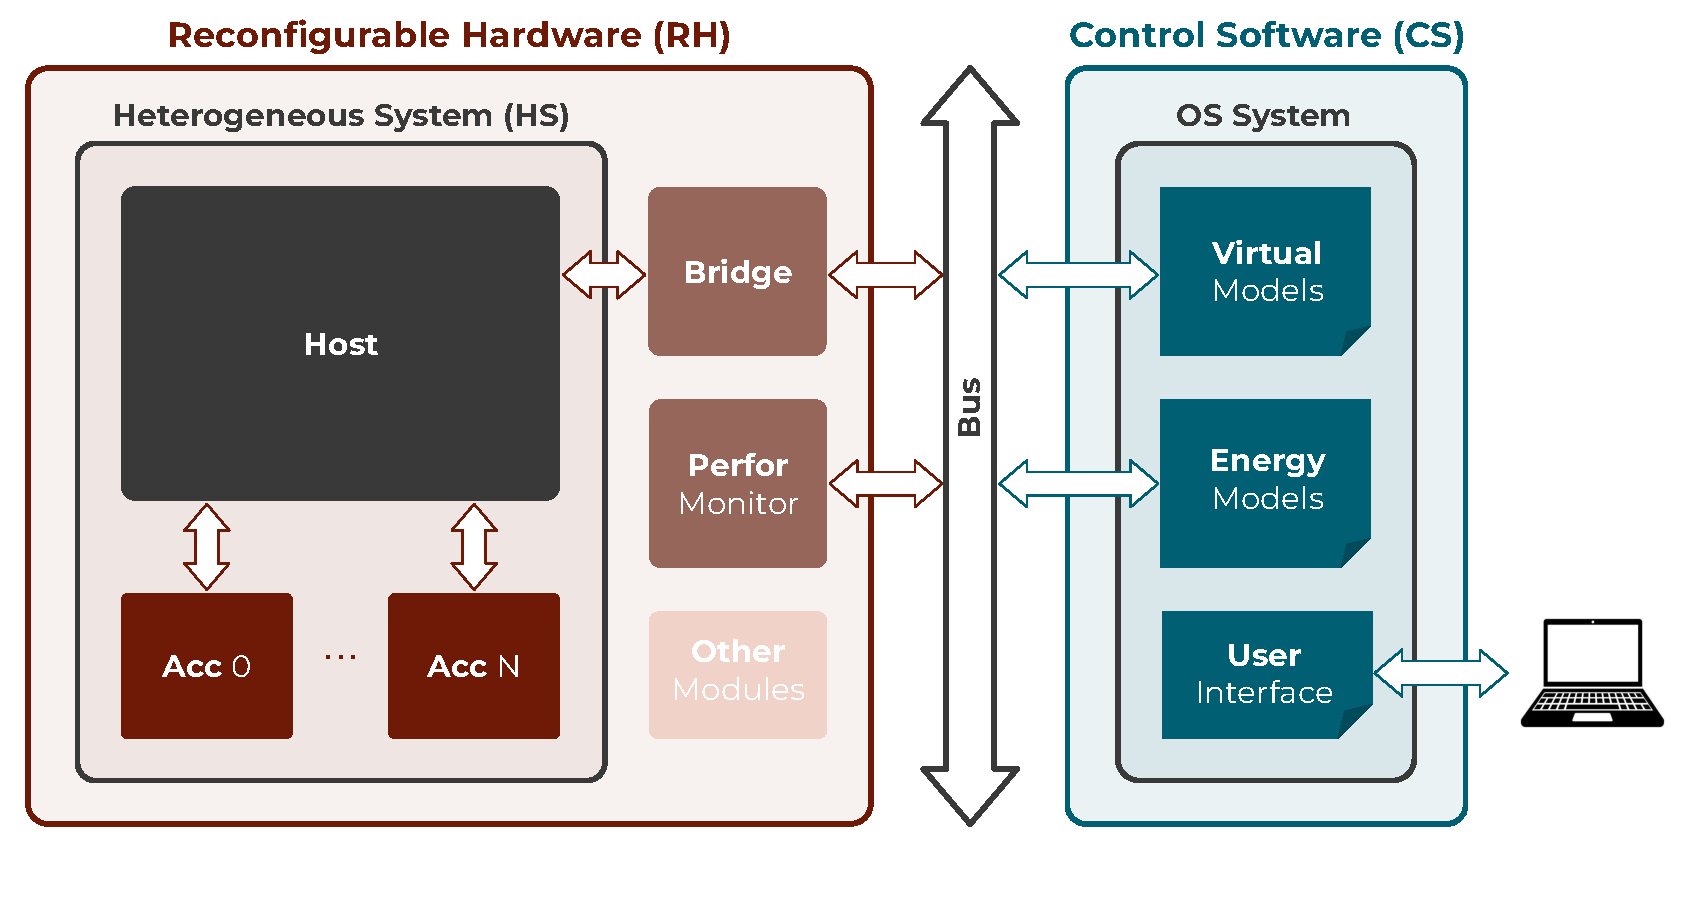
\includegraphics[width=0.8\textwidth]{figures_femu/femu_blocks.pdf}
                \caption{Block diagram of the \mbox{FEMU} framework for prototyping TinyAI heterogeneous systems.}
                \label{fig:femu_blocks}
            \end{figure}

            The \mbox{FEMU} framework is composed of a modular set of hardware and software components organized across two main regions: the RH region and the CS region. The following sections describe their roles and how they interact to enable virtualization, system monitoring, and development automation.

            \subsubsection{Prototyping Regions}
            
                Figure~\ref{fig:femu_blocks} describes the \mbox{FEMU} architecture. The RH region, implemented in the reconfigurable logic area of an SoC-based FPGA, hosts the heterogeneous system under development. Enabling direct deployment of RTL or high-level synthesized modules facilitates functional integration and cycle-accurate evaluation of processing elements in a modular fashion.
            
                Within the RH, the host subsystem typically includes a general-purpose CPU, private and shared memory banks, a system bus, and a variety of peripheral interfaces. This infrastructure replicates the structure of a real-world system, allowing end-to-end validation of both software and hardware components under realistic resource constraints. The system supports standard communication mechanisms for interacting with custom accelerators dedicated to the most critical kernels.
            
                To enhance its capabilities, the RH integrates a set of auxiliary modules. A dedicated bridge connects the RH to the CS, enabling data exchange and control signaling. This bridge is fundamental for virtualization, allowing the CS to emulate or supervise hardware behaviors without interfering with RH execution. Additionally, the RH includes a performance monitor that tracks runtime activity, providing fine-grained observability into application behavior and enabling accurate performance analysis.
            
                Complementing the RH, the CS region runs a lightweight operating system and hosts the runtime infrastructure required for system control and evaluation. This includes high-level software libraries that enable test orchestration, system monitoring, and communication with the RH. The CS provides a high degree of flexibility and automation, supporting dynamic reconfiguration, high-level debugging, and repeatable experiments without requiring manual board-level interaction.

            \subsubsection{Virtualization Infrastructure}
            
                A central feature of the framework is its comprehensive support for component virtualization. This abstraction layer enables software to emulate key system modules, including debuggers, ADCs, flash memories, and accelerators. By decoupling software development from hardware availability, virtualization accelerates early-stage development, enables functional validation before RTL completion, and supports rapid design-space exploration. It also allows development teams to work in parallel, reducing integration overhead and streamlining co-design workflows.
            
                \subsubsection*{Debugger Virtualization}
                
                    Debugger virtualization enables the CS to take full control of the RH execution environment, eliminating the need for external programming tools or debuggers. Through a high-level interface, developers can load firmware into the RH, control program execution, inspect internal registers and memory states, and retrieve outputs. This is achieved via lightweight communication between the CS and RH, abstracting low-level debug signals and exposing unified access to the developer.
                    
                    This infrastructure supports automated test campaigns and continuous integration by allowing seamless reprogramming, debugging, and validation through scripts. Developers can automate the execution of multiple application variants, collect results, and analyze errors or performance regressions, all from a single script running on the CS. This drastically reduces iteration time and improves productivity, especially in early prototyping phases, where bugs and design changes are frequent. As a result, debugger virtualization plays a crucial role in shortening the development cycle and improving the reliability of the system.
                
                \subsubsection*{ADC Virtualization}
                
                    ADC virtualization provides a realistic and efficient emulation of real-time sensor data acquisition without requiring physical analog interfaces or signal generators. In many TinyAI applications, data collection is tightly coupled to the operation of analog front-ends and ADCs, which are expensive and inflexible to integrate during early development. \mbox{FEMU} addresses this limitation by streaming pre-recorded datasets into the RH using a time-synchronized delivery mechanism that replicates the behavior of actual ADC sampling.
                    
                    This is implemented using a dual-buffered data structure. A software-controlled circular buffer transfers samples from a large external storage to the CS memory. In parallel, a hardware-managed buffer moves data from the CS memory to the RH, making it available to the heterogeneous system. The mechanism enables developers to precisely emulate scenarios with various acquisition rates, allowing for the evaluation of performance and energy under realistic timing constraints. Moreover, using real signal datasets enables functional validation of the entire acquisition-processing pipeline, making this virtualization strategy essential for validating applications such as biomedical monitoring or audio inference before hardware integration.
                
                \subsubsection*{Flash Virtualization}
                    
                    Flash virtualization provides a high-throughput, software-driven abstraction of non-volatile storage. In embedded systems, accessing flash memory typically involves long latencies, restricted bandwidth, and limited write endurance, factors that hinder rapid development and testing. The \mbox{FEMU} framework overcomes these constraints by emulating flash storage using fast and large memory available in the CS region.
                    
                    This approach supports both read and write transactions and allows the emulated flash to store input datasets, model parameters, test vectors, and result logs. Input files can be pre-loaded into CS memory and made accessible to the RH at runtime, reducing test setup time and enabling fast experimentation. Write-back capability allows applications to store intermediate results or logs without physically wearing out the flash, facilitating long-running debug sessions and functional tracing.
                    
                    This abstraction is particularly useful in iterative workflows such as machine learning inference and testing, where large volumes of data are processed repeatedly. By decoupling flash behavior from physical devices, the virtualization layer enables flexibility, scalability, and simplified test automation, making it a vital tool for comprehensive application development.
                
                \subsubsection*{Accelerator Virtualization}
                
                    Accelerator virtualization enables the integration of hardware accelerators into the development flow even before their RTL implementations are available. This is accomplished by describing accelerators as software models that execute on the CS and respond to memory-mapped register interactions as if they were physical hardware components in the RH. From the perspective of the application running on the host, the interface and behavior of the accelerator remain unchanged.
                    
                    This mechanism provides multiple benefits. It allows software developers to write and test application code that interfaces with the accelerator through the same functions and communication protocols that will be used in the final implementation. This reduces the likelihood of integration bugs and allows bottlenecks to be identified and addressed early. Furthermore, it enables architectural experimentation by modifying the internal behavior, latency, or output characteristics of the model.
                    
                    From a project management perspective, accelerator virtualization supports hardware/software parallelism. Hardware designers can iterate on RTL development while software engineers test functionality and validate use cases, thus minimizing development stalls. The result is a faster, more collaborative, and more resilient co-design process, especially important in time-constrained or resource-limited research environments.
            
            \subsubsection{Energy Estimation Infrastructure}
            
                Energy efficiency is a critical design metric in TinyAI systems, where devices often operate on small batteries or harvest energy from the environment. To support energy-aware development, \mbox{FEMU} includes an integrated energy estimation infrastructure that links runtime activity with technology-specific energy models. This allows the framework to deliver realistic energy consumption estimates without relying on physical measurement tools.
                
                The process begins with runtime monitoring, where the RH collects performance metrics during program execution. These metrics are then relayed to the CS and combined with energy models derived from silicon implementations. These models capture the power costs of various modules under different voltage, frequency, and process conditions.
                
                The result is a detailed energy breakdown that allows developers to assess the cost of each subsystem or application phase, such as acquisition and processing. Developers can evaluate trade-offs between software and hardware acceleration or compare alternative accelerator implementations for energy savings. This capability is particularly valuable in the early stages of design exploration, where architectural decisions have a strong impact on system efficiency.
            
            \subsubsection{User Interface and Automation}
            
                To make all features of the framework accessible and usable, \mbox{FEMU} provides a high-level user interface, which abstracts complex system-level operations and exposes a consistent set of commands for controlling all aspects of the system. Developers can compile and run applications, start and stop debug sessions, collect performance data, and invoke energy estimation routines, all from a single control interface.
                
                The interface supports both interactive and scripted usage. It can be used manually during development or integrated into automated workflows, enabling batch testing, regression checking, and large-scale design-space exploration. By lowering the entry barrier and reducing the friction associated with FPGA-based prototyping, the interface plays a key role in the usability and scalability of the \mbox{FEMU} framework.

        \subsection{Prototyping and Evaluation Flow}
        
            Figure~\ref{fig:femu_flow} illustrates the iterative prototyping and evaluation cycle supported by the \mbox{FEMU} framework. This flow is designed to guide the hardware/software co-design of TinyAI heterogeneous systems, with a particular focus on identifying, integrating, and optimizing hardware accelerators for compute-intensive tasks. The process emphasizes end-to-end system validation and energy-performance trade-off analysis, enabling developers to build optimized platforms tailored to ultra-low-power constraints.

            \subsubsection*{Prepare Application}
            
                The process begins with the selection and preparation of the target application. This application typically originates from a domain-specific workload such as biomedical signal processing, environmental monitoring, or on-device machine learning, where performance and energy constraints are critical. The application is first analyzed and optimized in software based on system-level constraints, including latency, throughput, memory footprint, and power budget. These initial considerations ensure that the design space exploration focuses on the most relevant bottlenecks and performance objectives.
            
            \subsubsection*{Application Profiling}
            
                Once the application is functionally complete and verified in software, it is executed entirely on the host CPU implemented in the RH region~(Step~1). During this run, the system collects detailed performance statistics using the built-in monitoring infrastructure. Simultaneously, energy consumption is estimated using the integrated energy modeling capabilities, providing a quantitative baseline for the CPU-only execution. This step serves as the performance and energy reference against which future accelerator-based enhancements are evaluated.
            
            \subsubsection*{Candidate Kernel Identification}
            
                The second step focuses on identifying the most computationally intensive kernels within the application~(Step~2). Using the collected profiling data, the framework provides utilities for dynamic analysis to identify hotspots, which are the sections of the code that contribute disproportionately to execution time or energy consumption. These bottlenecks are often suitable candidates for hardware acceleration, provided that they exhibit sufficient regularity, data reuse, or parallelism. Identifying the right kernel to accelerate is crucial for maximizing the efficiency of the hardware design effort.

                \begin{figure}[t]
                    \centering
                    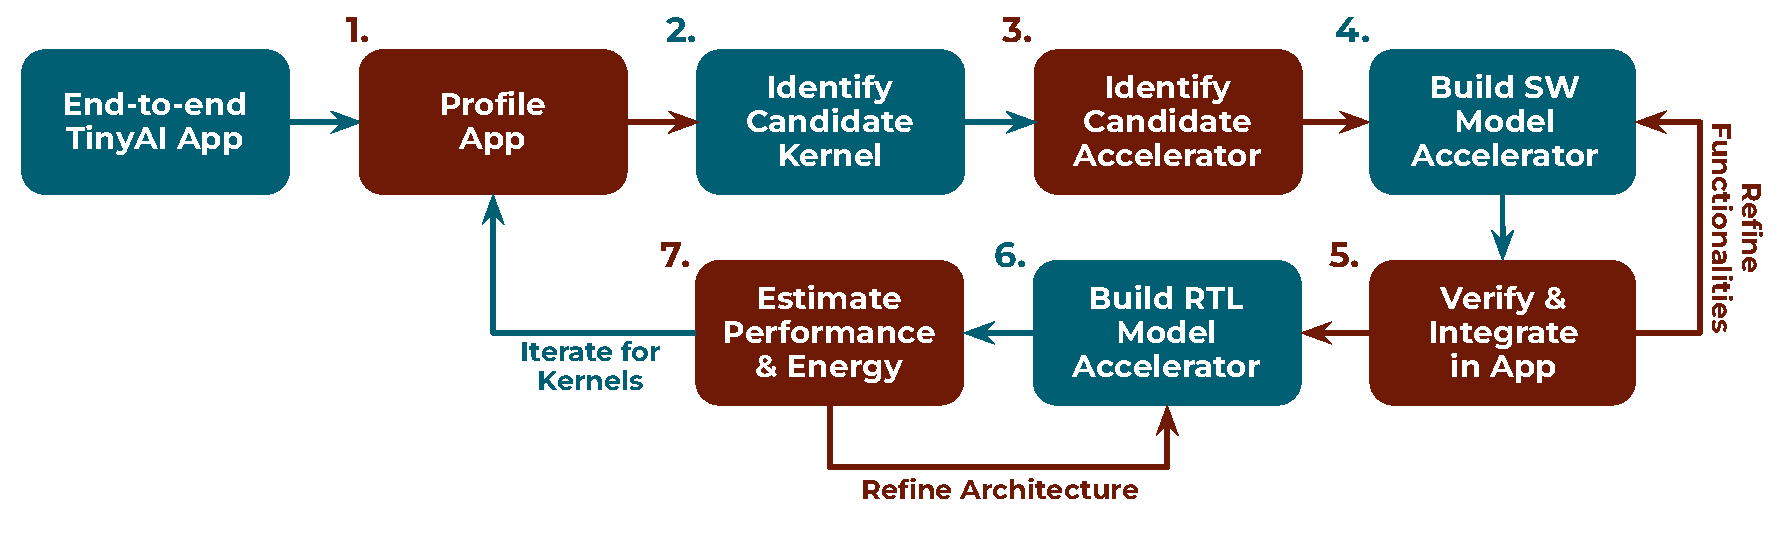
\includegraphics[width=1\textwidth]{./figures_femu/femu_flow.pdf}
                    \caption{Design cycle for prototyping and evaluating TinyAI accelerators.}
                    \label{fig:femu_flow}
                \end{figure}
            
            \subsubsection*{Candidate Accelerator Selection}
            
                Once a suitable kernel is selected, the third step involves identifying the type of accelerator most appropriate for implementing it in hardware~(Step~3). The decision may involve choosing among specialized datapaths, configurable SIMD engines, or domain-specific units, depending on the computational pattern of the kernel. This phase relies on the designer expertise and prior architectural knowledge to guide the choice of accelerator type. This step bridges profiling analysis with architectural design by defining accelerator requirements in terms of functionality, latency, and memory access behavior.
            
            \subsubsection*{Accelerator Software Modeling}
            
                With a clear target in mind, the developer implements a high-level software model of the selected accelerator~(Step~4). This model is typically written in a high-level programming language and is deployed within the CS region using the virtualization infrastructure. The accelerator model is exposed to the application via the same memory-mapped interface that will be used by the final RTL module, allowing seamless integration without changes to the host software. This step enables early testing and rapid functional validation without committing to a hardware implementation.
            
            \subsubsection*{Functional Validation}
            
                The functional correctness of the virtualized accelerator is then verified~(Step~5). The application is re-executed, this time with the software model of the accelerator replacing the original kernel. The output of the application is compared against the CPU-only baseline to ensure bit-accurate consistency. This validation ensures that offloading to hardware does not compromise the correctness of the application logic, and it enables iterative refinement of the interface and behavior of the accelerator model before hardware realization. The modularity of FEMU simplifies this substitution process and accelerates the transition from virtual to physical integration.
            
            \subsubsection*{Accelerator RTL Implementation}
            
                Once the virtualized model is validated, the design proceeds to hardware implementation~(Step~6). The software model is either manually translated into a hardware description language (e.g., Verilog or VHDL) or synthesized using high-level synthesis (HLS) tools to generate an RTL implementation. The accelerator is then integrated into the RH region along with the host system, typically as a memory-mapped peripheral on the system bus. The integration process is facilitated by the modular structure of \mbox{FEMU}, which allows seamless reconfiguration of the RH without affecting the CS or other software components.
            
            \subsubsection*{Performance and Energy Estimation}
            
                After integration, the accelerator is evaluated in hardware to collect updated performance metrics and estimate system-level energy efficiency~(Step~7). The application is executed with the accelerator, which is now implemented in RTL and deployed in the RH, and performance is collected using the monitoring infrastructure. This enables a comparison with the CPU-only baseline, revealing the latency and throughput improvements achieved through hardware offloading. At the same time, the RTL implementation undergoes synthesis, place-and-route, and dynamic power analysis using commercial EDA tools. These tools extract technology-specific power values that are then used as building blocks to form the energy model of the new accelerator and estimate the overall energy efficiency.
            
            \subsubsection*{Design Refinement}
            
                The obtained quantitative results inform the next refinement phase, where architectural adjustments may be applied to further optimize the accelerator design. This could involve modifying data widths, optimizing memory interfaces, or restructuring the datapath. These refinements are iteratively applied to maximize energy efficiency or better meet the timing constraints of the application. The integration of refinement as a core part of the flow ensures that accelerator development is not a one-shot process, but a feedback-driven cycle.
            
            \subsubsection*{Kernel Iteration}
            
                Finally, the framework supports the reuse of this flow across multiple kernels within the same application. Once a single kernel is optimized, developers can loop back to identify and accelerate additional bottlenecks. This iterative methodology allows developers to progressively improve the overall performance and energy profile of their TinyAI system through targeted acceleration and architectural tuning. Over time, this results in a highly optimized heterogeneous system tailored to the computational profile of the application.
            
            Through this structured and iterative methodology, the \mbox{FEMU} framework supports efficient co-design and quantitative evaluation of TinyAI systems. It enables developers to explore multiple architectural choices with minimal overhead, identify bottlenecks early, and converge toward optimized designs that meet the stringent performance and energy requirements of this domain.

    \section{An Implementation}
    \label{sec:an_implementation}
    
        This section presents a concrete instantiation of the \mbox{FEMU} framework, realized using commercially available hardware and software components. The goal of this implementation is to demonstrate the practical feasibility and versatility of the framework when applied to real-world scenarios. The resulting platform, referred to as \mbox{X-HEEP-FEMU}, serves as both a validation vehicle for the proposed methodology and a ready-to-use reference design for future TinyAI research and development.
        
        The \mbox{X-HEEP-FEMU} platform closely follows the prototyping and evaluation flow described in Section~\ref{sec:the_framework}, covering all key functionalities: integration of a heterogeneous system in the RH, deployment of virtualization infrastructure, performance and energy evaluation, and support for end-to-end development and testing of TinyAI applications. Importantly, this section also illustrates how each architectural block described in Figure~\ref{fig:femu_blocks} can be instantiated with specific real-world components.
        
        As a reusable research platform, \mbox{X-HEEP-FEMU} highlights how the \mbox{FEMU} framework can be customized and extended to match different system constraints, target applications, and energy-performance goals. The design choices made in this case study, ranging from the selected host to the interfacing logic and runtime environment, were driven by the need to balance fidelity, flexibility, and resource usage, while maintaining a realistic execution model representative of emerging TinyAI devices.
        
        Figures~\ref{fig:x-heep-femu_pl} and~\ref{fig:x-heep-femu_ps} illustrate the complete block diagram of the \mbox{X-HEEP-FEMU} instantiation, highlighting the interplay between the RH and CS components. Each block corresponds to a concrete implementation mapped to specific FPGA resources or software layers. The description in the following sections is organized according to the structured methodology adopted during the development of the platform.

        \begin{figure} [t]
            \centering
            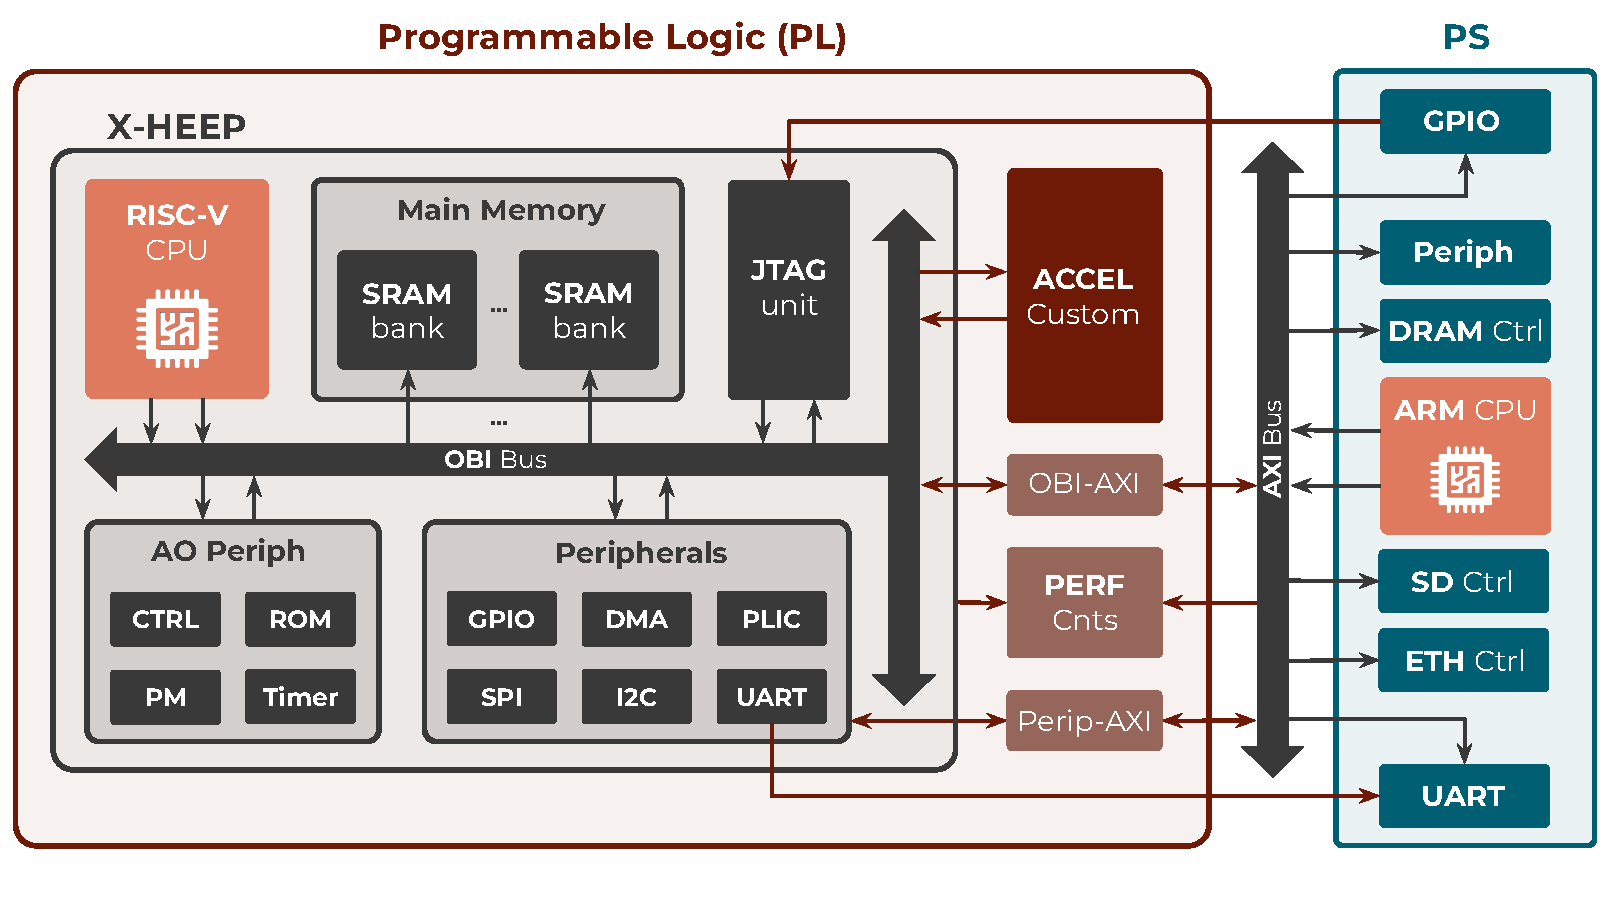
\includegraphics[width=1\textwidth]{./figures_femu/x-heep_femu_pl.pdf}
            \caption{Block diagram of the \mbox{X-HEEP-FEMU} platform focusing on the programmable logic, implemented on the Xilinx Zynq-7020 on the Pynq-Z2 board.}
            \label{fig:x-heep-femu_pl}
        \end{figure}

        \begin{figure} [t]
            \centering
            \includesvg[width=1\textwidth]{./figures_femu/x-heep_femu_ps.svg}
            \caption{Block diagram of the \mbox{X-HEEP-FEMU} platform focusing on the processing system, implemented on the Xilinx Zynq-7020 on the Pynq-Z2 board.}
            \label{fig:x-heep-femu_ps}
        \end{figure}

        \subsection{Choosing an SoC-Based FPGA and Host}
        
            The first step in instantiating the \mbox{FEMU} framework involves the careful selection of a suitable SoC-based FPGA platform capable of supporting both hardware prototyping and software-driven system control. This decision must account for several design criteria, including hardware flexibility, software compatibility, performance, power consumption, and ease of use. These criteria are particularly critical when targeting TinyAI systems, where real-time performance must be balanced with stringent energy and area constraints.
            
            To meet these requirements, the Xilinx Zynq-7020 SoC integrated on the Pynq-Z2 development board~\cite{pynq-z2} is selected, with its main features summarized in Table~\ref{tbl:zynq7020}. This platform provides an effective balance of hardware resources, software flexibility, and cost efficiency, making it well-suited for early-stage system prototyping and academic research.
            
            The Zynq-7020 device combines two fundamental components:

            \vspace{-1em}
            \begin{itemize}
                \item \textbf{Programmable Logic (PL)}: This reconfigurable region serves as the RH in our framework. It enables the implementation of custom digital logic, including the under-development heterogeneous system and additional infrastructure. The PL offers sufficient logic cells, block RAM, and DSP slices to host a complete SoC prototype with moderate complexity.
                
                \item \textbf{Processing System (PS)}: This processing region serves as the CS in our framework. It integrates a dual-core ARM Cortex-A9 processor operating at up to \SI{667}{\mega\hertz}, along with on-chip peripherals and memory interfaces. This subsystem provides an environment for software-driven control, application orchestration, debugging, and energy-performance monitoring. The Cortex-A9 cores are capable of running a full Linux operating system, enabling high-level software development and remote automation.\\\\
            \end{itemize}
            \vspace{-1em}
            
            To host the software stack, a custom \mbox{Ubuntu} image~\cite{sd_image} is deployed on the PS, chosen for its lightweight footprint, broad package support, and compatibility with embedded hardware. Ubuntu provides a robust environment for running Python scripts, interacting with device drivers, and integrating third-party software tools needed for full-system evaluation. The open nature of the distribution also allows developers to tailor kernel and boot-loader configurations to the specific constraints of the platform.

            \begin{table}[tp]
                \caption{Summary of the features of the Xilinx Zynq-7020 SoC on the Pynq-Z2 board.}
                \label{tbl:zynq7020}
                \centering
                \resizebox{0.9\textwidth}{!}{
                \begin{tabular}{|l|l|}
                \toprule
                \bf{Component} & \bf{Description} \\
                \midrule
                \textbf{Processing System (PS)} & Dual-core ARM Cortex-A9 (up to \SI{866}{\mega\hertz}) \\
                & NEON SIMD engine and Vector Floating Point Unit \\
                & 512\,KB L2 cache, AXI interconnect to PL \\
                \midrule
                \textbf{Programmable Logic (PL)} & 85\,k logic cells (equivalent to Artix-7) \\
                & 220 DSP slices, 560\,KB BRAM, 53,200 LUTs \\
                & High-speed AXI interfaces to/from PS \\
                \midrule
                \textbf{On-Chip Memory} & 256\,KB On-Chip Memory (OCM) shared by PS \\
                \midrule
                \textbf{External Memory} & 512\,MB DDR3 RAM (\SI{1066}{\mega\hertz}, connected to PS) \\
                \midrule
                \textbf{Storage} & 16\,MB QSPI Flash (for boot image) \\
                & MicroSD card slot (used for Linux file system) \\
                \midrule
                \textbf{Connectivity} & 1\,Gbps Ethernet (via PS GEM interface) \\
                & USB OTG 2.0, UART, HDMI out (from PL) \\
                \midrule
                \textbf{Peripherals (Pynq-Z2)} & 2× Pmod ports (12-pin), Arduino shield header \\
                & 6× push buttons, 4× switches, 4× LEDs \\
                & Audio codec with microphone and line in/out \\
                \midrule
                \textbf{Power Supply} & USB or 12\,V external power jack \\
                \midrule
                \textbf{Clocking} & \SI{33.33}{\mega\hertz} system oscillator; multiple PLLs available \\
                \bottomrule
                \end{tabular}
                }
            \end{table}
            \vspace{+2em}
            
            The Pynq-Z2 board further complements these capabilities with essential peripherals for standalone operation and software deployment. 
            
            These include:

            \vspace{-1em}
            \begin{itemize}
                \item \textbf{A secure digital (SD)} card reader for booting the system and hosting persistent storage, including the Ubuntu root file-system and development tools.
                
                \item \textbf{\SI{512}{\mega\byte} of DDR3 DRAM} accessible by the PS, which is used to execute user applications, store performance logs, manage virtualization buffers, and host large datasets used for emulating acquisition and inference tasks.
                
                \item \textbf{An Ethernet interface} that provides network connectivity for remote development, file transfer, and integration with cloud-based development pipelines. This feature enables full remote access to the board, including reprogramming and test orchestration, eliminating the need for physical interaction during iterative development cycles.
            \end{itemize}
            % \vspace{-1em}
            
            After selecting the hardware platform, the next step is to choose a suitable host to instantiate within the PL. This host must provide a balance between simplicity, configurability, and extensibility to support the integration of a diverse range of accelerators. For this purpose, the \mbox{X-HEEP}~\cite{x-heep} host is adopted for its flexible design. 
            
            \mbox{X-HEEP} features a configurable architecture that includes a lightweight RISC-V core~\cite{zeroriscy}, tightly coupled data and instruction memory, an interconnect, and peripherals. Its modular and parameterized design makes it an excellent fit for rapid prototyping in TinyAI contexts. The platform also supports hardware extensions, allowing developers to seamlessly integrate accelerators and custom peripherals within a cohesive system architecture. The input/output interfaces of \mbox{X-HEEP} that are not used internally by \mbox{X-HEEP-FEMU} are routed to the board connectors, with the corresponding pinout shown in Figure~\ref{fig:pinout}.
            
            Together, the Pynq-Z2 board and the \mbox{X-HEEP} host form the hardware foundation of the \mbox{X-HEEP-FEMU} platform, enabling realistic emulation of TinyAI workloads while providing the flexibility and observability required for performance and energy-aware design exploration.

        \subsection{Setting up a Virtualization Strategy}
        
            Once the SoC-based FPGA and the hardware host are selected, the next critical step in realizing a functional \mbox{FEMU} instantiation is defining and deploying a comprehensive virtualization strategy. This strategy is central to the ability of the framework to decouple hardware and software development, simplify integration and testing, and enable early-stage validation of system functionalities. Specifically, virtualization abstracts key system components by replicating their behavior through software running on the PS, in conjunction with lightweight hardware infrastructure deployed in the PL.
            
            The virtualization scheme is designed to preserve the timing behavior, dataflow semantics, and control interfaces of the actual hardware, thereby ensuring high-fidelity emulation of the system under development. The following descriptions detail how each component is virtualized within the \mbox{X-HEEP-FEMU} platform and explain how the PS and PL regions interact to emulate realistic system behavior without requiring physical peripherals or external instrumentation.

            \begin{figure} [t]
                \centering
                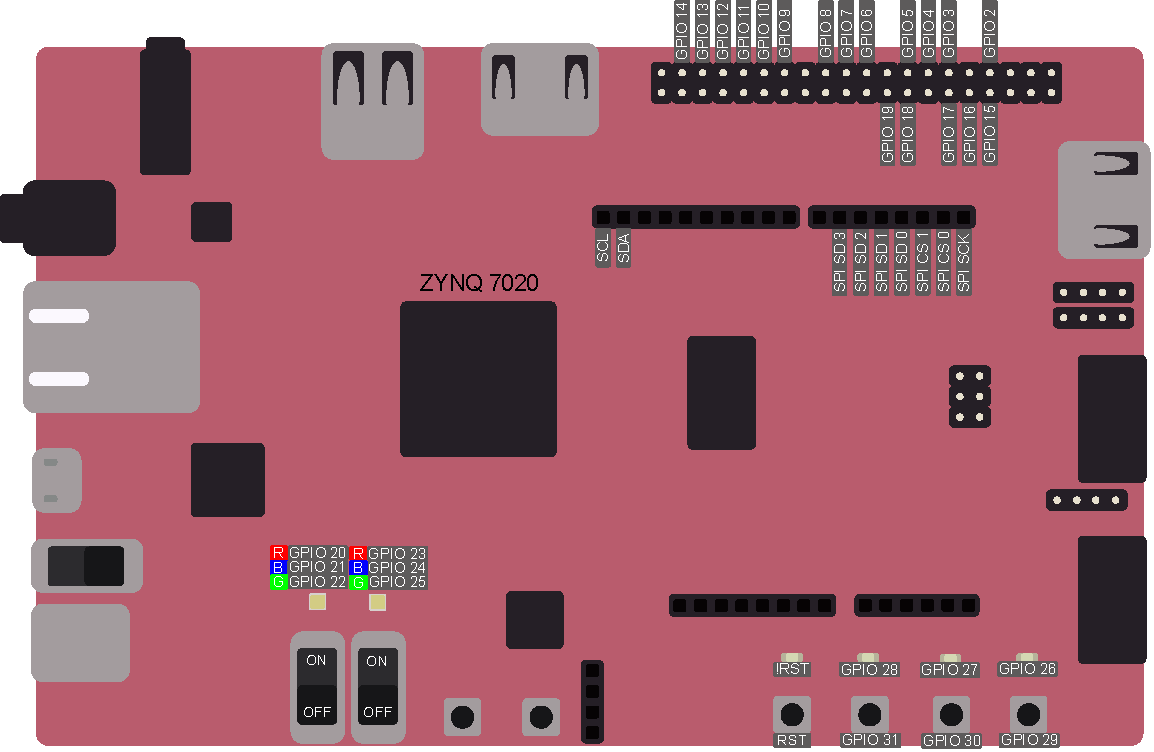
\includegraphics[width=0.8\textwidth]{./figures_femu/pinout.pdf}
                \caption{Pinout of the Pynq-Z2 board.}
                \label{fig:pinout}
            \end{figure}
            
            \subsubsection*{Debugger Virtualization}
            
                To streamline software development and automate application testing, the platform implements a fully virtualized debugging infrastructure. The \mbox{X-HEEP} host includes a JTAG interface, which is typically accessed through an external debugger. Instead, in \mbox{X-HEEP-FEMU}, the JTAG signals are connected to general-purpose input/output (GPIO) pins exposed by the PS and routed through the PL. This setup enables the PS to control the JTAG interface using standard debugging tools directly.
                
                The GNU Debugger (GDB) is employed as the front-end interface, while OpenOCD acts as a middleware server. OpenOCD translates GDB commands into JTAG signals and drives the GPIO lines accordingly, effectively allowing step-by-step execution, register inspection, and memory manipulation from within the Linux environment on the PS. This eliminates the need for external debug hardware, allowing for the full automation of software flashing, execution, and verification through scripting.
                
                In parallel, the UART peripheral of the \mbox{X-HEEP} host is connected to a UART interface available on the PS. This enables bidirectional communication between the application running on \mbox{X-HEEP} and the user-space tools on the PS, facilitating log-in, command input, and interactive debugging using standard terminal emulators.
        
            \subsubsection*{ADC \& Flash Virtualization}
            
                Sensor emulation is essential for evaluating acquisition-intensive workloads in TinyAI applications. To replicate real-time sensor sampling behavior, \mbox{X-HEEP-FEMU} employs a two-stage ADC virtualization mechanism that streams pre-recorded data samples from memory.
                
                On the hardware side, an SPI-to-AXI bridge is instantiated in the PL. This bridge translates serial peripheral interface (SPI) requests issued by the \mbox{X-HEEP} host into Advanced eXtensible Interface (AXI) transactions that fetch data from a hardware first-in first-out (FIFO). The FIFO is preloaded with data from the PS DRAM, ensuring compliance with the timing constraints expected by the host. The bridge is also memory-mapped into the PS address space, allowing for simple configuration and runtime control.
                
                Complementing the hardware pipeline, a software-controlled FIFO operates on the PS. It continuously streams pre-recorded signal data from an SD card into DRAM, preloading complete acquisition windows in advance.
                
                Together, hardware and software FIFOs form a pipelined data path that guarantees continuous data delivery to the heterogeneous system, minimizing latency. This setup accurately mimics real-world ADC sampling while enabling validation with complex and realistic datasets.
                
                In parallel, \mbox{X-HEEP-FEMU} supports non-volatile storage emulation through a second instance of the same SPI-to-AXI bridge. This virtual flash interface is configured to support both read and write transactions, providing a flexible and high-performance mechanism for bulk data exchange between the heterogeneous system and DRAM.
                
                By decoupling memory access from the limitations of physical flash devices, such as long access latencies, restricted bandwidth, and limited write endurance, this virtualized interface enables high-throughput access to large datasets. As a result, developers can evaluate and iterate on memory-intensive TinyAI workloads efficiently, minimizing bottlenecks.
            
            \subsubsection*{Accelerators Virtualization}
            
                Virtualization of hardware accelerators is another feature of the \mbox{FEMU} framework. In early-stage design, it is often necessary to evaluate software-hardware offloading strategies before RTL implementations of accelerators are available. To support this, the platform emulates accelerator behavior entirely in software within the PS.
                
                This is achieved by reserving memory-mapped regions in DRAM that are accessible to both the PS and the PL. The \mbox{X-HEEP} host writes configuration parameters and input data to this shared memory via an OBI-to-AXI bridge, connected to the PS. A software thread running on the PS continuously monitors the memory region for transaction requests. Upon detection, it executes the corresponding kernel in software, using a high-level model of the accelerator, and writes the output back to a dedicated output memory region.
                
                From the perspective of the host, this interaction is indistinguishable from communicating with a real hardware accelerator mapped to the PL. The same interface, handshaking protocol, and memory layout are preserved, allowing seamless migration from virtual to RTL-based accelerators in later stages of the development flow.

        \subsection{Setting up a Performance Estimation Strategy}
        
            A key requirement in the development and evaluation of TinyAI systems is the ability to accurately measure system performance at runtime. Such measurements enable developers to identify computational bottlenecks, analyze power-state behavior, and compare different implementations (e.g., software vs. hardware acceleration) based on quantitative evidence. To support this, the \mbox{X-HEEP-FEMU} platform integrates a customizable performance estimation infrastructure within the PL.

            \subsubsection*{Performance Counters}
            
                At the heart of this infrastructure is a set of lightweight performance counters specifically designed to monitor activity across key system domains. These counters track the evolution of control signals, such as clock enable, power enable, and memory retention flags, which collectively indicate the operational state of each domain. 
                
                In particular, the counters measure the number of clock cycles that each monitored domain spends in one of the following four power states:

                \vspace{-1em}
                \begin{itemize}
                    \item \textbf{Active}: the domain is fully powered and clocked, performing computation.
                    \item \textbf{Clock-gated}: the domain is powered, but the clock is disabled to minimize dynamic power.
                    \item \textbf{Power-gated}: the domain is completely shut down to save leakage power.
                    \item \textbf{Retention}: specific to memories, where the cell content is retained with minimal power while disabling both read/write access and clocks.
                \end{itemize}
                \vspace{-1em}

                This power-state classification provides a granular view of how system resources are utilized during application execution. This is particularly useful for understanding energy-efficiency trade-offs and optimizing duty cycles in ultra-low power regimes.
                
                To accommodate different usage scenarios, the performance counters support two complementary operating modes:

                \vspace{-1em}
                \begin{itemize}
                    \item \textbf{Automatic mode}: In this configuration, counters are implicitly triggered at the start and end of the application execution. Trigger signals are generated automatically and do not require developer intervention. This mode is ideal for whole-application profiling, providing a straightforward mechanism for collecting end-to-end metrics over a complete workload.
                
                    \item \textbf{Manual mode}: This configuration gives developers fine-grained control over the measurement window by enabling or disabling counters via a dedicated GPIO signal. The application software can raise or lower this signal at runtime to demarcate specific code regions for profiling. This capability is particularly useful for analyzing compute kernels, memory access patterns, and I/O transactions in isolation, facilitating detailed bottleneck analysis and local optimizations.
                \end{itemize}
                \vspace{-1em}
                
                Overall, performance counters are memory-mapped onto the AXI bus, making them directly accessible from the control software running in the PS. Configuration registers allow developers to select which domains to monitor, reset counters, or enable/disable specific monitoring features. Counter values can be read via user-space scripts or integrated into performance logging pipelines for post-execution analysis.
                
            \subsubsection*{Accelerator Monitoring}
            
                When accelerators are integrated into the PL as RTL modules, additional performance counters can be instantiated specifically for their subdomains. These accelerator-specific monitors track usage metrics, such as active cycles and idle periods. This enables developers to quantitatively assess the accelerator runtime behavior and compare it to its software counterpart.
                
                Because the same classification of power states is maintained across all system components, CPU, memory, and accelerators, the framework supports unified performance analysis across the entire heterogeneous system. Developers can, for instance, compare the number of active cycles consumed by a task when executed on the CPU versus offloaded to an accelerator, and correlate this data with energy estimates derived from corresponding energy models.

        \subsection{Setting up an Energy Estimation Strategy}
        
            In energy-constrained domains such as TinyAI, achieving optimal performance is not sufficient. Energy efficiency must also be rigorously evaluated and optimized throughout the development process. Therefore, a critical component of the \mbox{FEMU} framework is its ability to estimate application-level energy consumption based on runtime performance data and technology-specific energy models. This capability enables designers to make informed architectural and algorithmic decisions early in the design flow, without requiring post-silicon measurements or expensive full-chip simulations.
            
            The overall energy estimation process is structured into three stages:

            \vspace{-1em}
            \begin{enumerate}
                \item \textbf{Power modeling}: The creation of accurate power models for individual components based on synthesis or post-layout data.
                \item \textbf{Runtime profiling}: The collection of real-time activity data from hardware counters and software instrumentation during system execution.
                \item \textbf{Model integration}: The computation of energy estimates by combining power models with the collected runtime activity.
            \end{enumerate}
            \vspace{-1em}
            
            This section outlines each stage and describes how the \mbox{X-HEEP-FEMU} platform implements them using a hybrid software/hardware approach.

            \subsubsection*{Power Modeling}
            
                At the foundation of this methodology lies a pre-characterized power model derived from a real silicon implementation of the \mbox{X-HEEP} host fabricated in TSMC \SI{65}{\nano\meter} CMOS technology. This silicon SoC, referred to as \mbox{HEEPocrates}~\cite{heepocrates}, was thoroughly characterized using silicon measurements to extract accurate average power values for each functional domain under four distinct power states: active, clock-gated, power-gated, and retention. These values serve as input parameters to the estimation engine.
            
            \subsubsection*{Runtime Profiling}
            
                During application execution, the performance counters previously described track the number of clock cycles each domain spends in each of the four power states. At the end of execution, the PS retrieves these counter values via the AXI interface and makes them available to the energy estimation engine.
                
                Let \( P_{d,s} \) denote the average power consumed by domain \( d \) in state \( s \), and \( T_{d,s} \) the time spent in that state as measured by the counters (in clock cycles). The energy consumption \( E_d \) for domain \( d \) is then given by:

                \vspace{-2em}
                \begin{equation}
                    E_d = \sum_{s \in \{a, cg, pg, r\}} P_{d,s} \cdot T_{d,s} \cdot T_{\text{clk}}
                \end{equation}
                \vspace{-2em}
                
                where \( T_{\text{clk}} \) is the clock period in seconds, and \( s \in \{a, cg, pg, r\} \) refers to the active, clock-gated, power-gated, and retention states, respectively. The total energy \( E_{\text{total}} \) consumed by the system is obtained by summing the contributions of all monitored domains:

                \vspace{-2em}
                \begin{equation}
                    E_{\text{total}} = \sum_d E_d
                \end{equation}
                \vspace{-2em}
                
                This energy estimation is computed on the PS after the execution completes and does not interfere with the target application timing, thus preserving the fidelity of runtime measurements.
            
            \subsubsection*{Accelerator Model Integration}
            
                In addition to host domains, the framework supports the integration of hardware accelerators. When these are realized as RTL modules, they are equipped with local performance counters that track their activity and power states. To estimate their energy contribution, developers must characterize the accelerator using standard EDA flows, e.g., synthesis, place-and-route, and power analysis, targeting the same technology node used for the host model (e.g., TSMC \SI{65}{\nano\meter}).

                Recognizing the variability of power characteristics across different standard-cell libraries and process-voltage-temperature (PVT) corners, the framework also supports the use of multiple power models. For instance, developers can define separate models for high-voltage threshold (HVT), standard-voltage threshold (SVT), and low-voltage threshold (LVT) libraries, or compare power consumption across different technology nodes (e.g., \SI{65}{\nano\meter} vs. \SI{22}{\nano\meter}).
                
                The resulting power model of the accelerator is then added to the system energy estimation infrastructure. The same runtime counter methodology is applied to determine time spent in each state, and total energy consumption is calculated accordingly. This modular integration supports flexible evaluation of alternative hardware acceleration strategies, enabling fine-grained comparisons between different implementations.

                \begin{figure} [t]
                    \centering
                    
\includegraphics[width=0.9\textwidth]{./figures_femu/snippet.png}
                    \caption{Code snippet of an HelloWorld application using the proposed \mbox{X-HEEP} Python class from Jupyter Notebooks.}
                    \label{fig:code}
                \end{figure}

        % \vspace{-1em}
        \subsection{Setting up a User Interface}
        
            The final component of the \mbox{X-HEEP-FEMU} implementation involves defining a user-friendly and flexible interface to interact with the emulation platform. Given the complexity of managing low-level hardware modules, virtualization mechanisms, and performance and energy infrastructure, an intuitive and high-level abstraction layer is crucial to ensure accessibility and productivity, particularly for software developers or system architects without an extensive hardware background.

            \subsubsection*{Dedicated Python Class}
            
                To this end, the platform offers a Python-based interface that encapsulates all low-level interactions with the platform into a structured and object-oriented software application programming interface (API). This interface is organized as a dedicated Python class \textit{X-HEEP} that exposes methods for each major functionality of the framework, including:

                \vspace{-1em}
                \begin{itemize}
                    \item Programming the PL with a specified bitstream.
                    
                    \item Compiling, loading, and executing applications on \mbox{X-HEEP}.
                    
                    \item Controlling debugger operations, such as breakpoints, step execution, and memory inspection.
                    
                    \item Managing virtualized components, such as streaming data to the ADC or reading/writing from virtual flash.
                    
                    \item Retrieving and parsing performance counter data from the PL.
                    
                    \item Performing energy estimation using pre-characterized models and runtime statistics.
                \end{itemize}
                \vspace{-1em}
            
                By abstracting these operations into simple function calls, the interface greatly reduces the learning curve and minimizes the potential for configuration errors during development. In addition, the class is written using modular and extensible design principles, making it easy to add new methods as the platform evolves. An example implementation of the \textit{HelloWorld} application is provided in the code snippet shown in Figure~\ref{fig:code}.
            
            \subsubsection*{Web-Based Interaction via Jupyter Notebooks}
            
                To further improve accessibility and encourage rapid experimentation, the Python interface is integrated with Jupyter Notebooks, enabling full interaction through a web browser. The Jupyter environment supports both command-line execution and visualization tools, making it ideal for interacting with embedded platforms in a graphical and scriptable manner.
                
                This integration transforms the \mbox{X-HEEP-FEMU} platform into a network-accessible design and evaluation tool. Any machine on the same network can connect to the Jupyter server using a standard HTTP browser, eliminating the need for physical access to the development board. This is particularly useful in shared lab environments or remote teaching scenarios, where multiple users may need access to the platform concurrently.
                
                Through the notebook interface, users can execute complete evaluation flows, including compilation, execution, profiling, and energy estimation, using just a few lines of Python code. Visualization libraries such as \texttt{matplotlib} or \texttt{seaborn} can be leveraged to plot performance and energy trends, further aiding in the analysis and reporting process.

    \section{Experimental Setup}
    \label{sec:experimental_setup}
    
        To validate the capabilities of the proposed \mbox{FEMU} framework and its implementation as the \mbox{X-HEEP-FEMU} platform, this section presents a structured set of experiments targeting representative use cases in the TinyAI domain. These experiments are designed to assess both the functional behavior and the performance-energy trade-offs of the system under realistic conditions, using complete application flows and real-world data.
        
        The primary objective of these experiments is to demonstrate that \mbox{X-HEEP-FEMU} supports accurate, repeatable, and flexible prototyping of TinyAI heterogeneous systems. In particular, the goal is to show that the platform can reproduce realistic acquisition and processing scenarios, support early-stage development through virtualization, and guide design decisions through reliable performance and energy estimation.
        
        To this end, the experimental evaluation is organized around three key use cases:

        \vspace{-1em}
        \begin{enumerate}
            \item \textbf{Signal acquisition characterization}: This experiment evaluates the behavior of the system during the data acquisition phase, particularly under varying sampling frequencies and memory buffering conditions. It demonstrates the accuracy and responsiveness of the presented ADC virtualization mechanism in replicating real-time sensor input behavior.
        
            \item \textbf{Computation of typical TinyAI workloads}: This use case evaluates the ability of the platform to execute representative compute-intensive tasks commonly found in TinyAI applications. It demonstrates how different implementations, including CPU-only and hardware-accelerated configurations, can be deployed, tested, and compared within the same development environment.
        
            \item \textbf{Sample collection and storage}: This experiment validates the presented flash virtualization strategy by simulating long-duration data logging and retrieval operations. It demonstrates the ability of the system to handle high-throughput memory transfers and emulate the behavior of real flash devices in terms of latency and bandwidth, without requiring physical storage. This experiment is based on a case study from the state-of-the-art~\cite{moisture}.
        \end{enumerate}
        \vspace{-1em}
        
        For each use case, the \mbox{X-HEEP-FEMU} platform is configured using its built-in interface to load the appropriate bitstream, virtualize the necessary components, and collect performance and energy data at runtime. Applications are executed in both CPU-only and hardware-accelerated configurations when applicable, allowing comparison between different system designs.

        \begin{table}[tp]
            \caption{Experimental setup for signal acquisition characterization on \mbox{X-HEEP-FEMU} and \mbox{HEEPocrates}.}
            \label{tbl:acquisition_setup}
            \centering
            \resizebox{0.85\textwidth}{!}{
            \begin{tabular}{|l|c|c|}
            \toprule
            \bf{Parameter} & \bf{X-HEEP-FEMU} & \bf{HEEPocrates} \\
            \midrule
            Acquisition Windows            & \SI{5}{\second} & \SI{5}{\second} \\
            Sampling Frequencies           & \SI{100}{\hertz}-\SI{100}{\kilo\hertz} & \SI{100}{\hertz}-\SI{100}{\kilo\hertz} \\
            Processing Element             & RISC-V CPU @ \SI{20}{\mega\hertz} & RISC-V CPU @ \SI{20}{\mega\hertz} \\
            Supply Voltage                 & - & \SI{0.8}{\volt} \\
            ADC Source                     & Virtualized ADC & On-board SPI \\
            Performance Estimation         & Performance Monitor & CPU Performance Counters \\
            Energy Estimation              & Energy model & Direct Measurement \\
            \bottomrule
            \end{tabular}
            }
        \end{table}

        \subsection{Signal acquisition characterization}
            
            The first use case evaluates the signal acquisition capabilities of the \mbox{X-HEEP-FEMU} platform by examining how the system performs when acquiring real-time sensor data under different sampling frequencies. This scenario reflects a common requirement in TinyAI applications, where sensor data must be collected at regular intervals and stored in memory for subsequent processing.
            
            In this experiment, a data acquisition kernel is executed on the \mbox{X-HEEP} CPU to capture a \SI{5}{\second} window of sensor samples via the SPI peripheral. Instead of interfacing with a physical ADC, the system employs the ADC virtualization infrastructure described in Section~\ref{sec:an_implementation}.
            
            To explore the impact of sampling frequency on system behavior, the acquisition kernel is executed across six different configurations: \SI{100}{\hertz}, \SI{500}{\hertz}, \SI{1}{\kilo\hertz}, \SI{10}{\kilo\hertz}, \SI{50}{\kilo\hertz}, and \SI{100}{\kilo\hertz}. These values span a broad spectrum of edge applications, from low-frequency physiological sensing (e.g., ECG, EEG) to high-frequency acoustic monitoring.
            
            During execution, the system tracks the runtime behavior using the performance monitoring infrastructure, and energy consumption is then estimated by combining the extracted data with the energy model derived from the \mbox{HEEPocrates} silicon implementation.
            
            To validate the fidelity of the emulation, the same acquisition kernel is executed on the physical \mbox{HEEPocrates} chip, configured at \SI{20}{\mega\hertz} and \SI{0.8}{\volt}. In this setup, data samples are retrieved from the on-board flash via SPI, replicating the same access pattern used in the emulated environment. Execution cycles are measured with CPU counters, and energy with power-rail instrumentation, enabling direct runtime and energy comparison between emulation and silicon.

        \subsection{Computation of Typical TinyAI Workloads}
        
            The second experimental use case focuses on characterizing the performance and energy efficiency of compute-intensive TinyAI workloads executed on both the general-purpose CPU and a hardware accelerator integrated within the \mbox{X-HEEP-FEMU} platform. These workloads are representative of fundamental operations found in many machine learning and signal processing pipelines and cover a broad spectrum of arithmetic intensity and memory access patterns:

            \vspace{-1em}
            \begin{itemize}
                \item \textbf{Matrix Multiplication (MM)}: a dense matrix-matrix product between a $121 \times 16$ matrix and a $16 \times 4$ matrix, using 32-bit integer (INT32) operands. This kernel reflects the core operation of many machine learning algorithms and is based on the setup in~\cite{najafi2024versasens}.
                
                \item \textbf{2D Convolution (CONV)}: a spatial convolution of a $16 \times 16$ input with three channels using eight filters of size $3 \times 3$, also in INT32. This operation is essential in CNN-based inference tasks and is implemented following~\cite{carpentieri2024performance}.
                
                \item \textbf{Fast Fourier Transform (FFT)}: a 512-point 1D transform executed using 32-bit fixed-point arithmetic (FxP32), following the workload structure proposed in~\cite{denkinger2022vwr2a}. FFT is a key workload in spectral analysis for biomedical and acoustic applications.
            \end{itemize}
            \vspace{-1em}
            
            Each kernel is evaluated under two different configurations:

            \vspace{-1em}
            \begin{enumerate}
                \item \textbf{CPU-only execution}: the kernel is compiled and executed directly on the \mbox{X-HEEP} RISC-V CPU. This configuration provides a software baseline for performance and energy consumption, serving as a reference point to quantify the benefits of hardware acceleration.
            
                \item \textbf{Accelerated execution with a CGRA}: the kernel is offloaded to a coarse-grained reconfigurable array (CGRA)~\cite{oe-cgra}, called \textit{OpenEdge CGRA}, which acts as a hardware accelerator tightly coupled with the host. The CGRA features a parameterizable tile-based architecture, with a dedicated configuration interface exposed through a slave open-bus interface (OBI) port and four master OBI ports for high-throughput memory access. This interface allows concurrent reads and writes from multiple banks of the \mbox{X-HEEP} main memory.
            \end{enumerate}
            \vspace{-1em}
            
            The accelerator integration follows a staged methodology. Initially, the CGRA is modeled as a Python software module within the PS, allowing early-stage validation of functionality, development of software drivers, and high-level debugging. This virtualized accelerator supports seamless testing and ensures behavioral correctness with minimal hardware overhead. Once validated, the same CGRA is implemented in RTL, mapped to the PL, and integrated with \mbox{X-HEEP} for unified performance and energy estimation.

            \begin{table}[tp]
                \caption{Experimental setup for evaluating TinyAI workloads on \mbox{X-HEEP-FEMU} and \mbox{HEEPocrates}.}
                \label{tbl:tinyai_workload_setup}
                \centering
                \resizebox{1\textwidth}{!}{
                \begin{tabular}{|l|c|c|}
                \toprule
                \bf{Parameter} & \bf{X-HEEP-FEMU} & \bf{HEEPocrates} \\
                \midrule
                Workloads & \multicolumn{2}{c|}{
                    \begin{tabular}[c]{@{}c@{}}
                    \textbf{Matrix Multiplication (MM)}: $121 \times 16 \times 4$ INT32 product \\
                    \textbf{2D Convolution (CONV)}: $16 \times 16 \times 3$ input, $3 \times 3 \times 8$ filters, INT32 \\
                    \textbf{Fast Fourier Transform (FFT)}: 512-point, fixed-point FxP32
                    \end{tabular}
                } \\
                \midrule
                Processing Elements & CPU-only, CGRA-accelerated & CPU-only, CGRA-accelerated \\
                Clock Frequency & \SI{20}{\mega\hertz} & \SI{20}{\mega\hertz} \\
                Supply Voltage & - & \SI{0.8}{\volt} \\
                Performance Estimation & Performance Monitor & CPU Performance Counters \\
                Energy Estimation & Energy Model & Direct Measurement \\
                \bottomrule
                \end{tabular}
                }
            \end{table}
            
            Performance measurement relies on the performance counters described in Section~\ref{sec:an_implementation}, which monitor both the CPU and the CGRA. For each power domain, the counters report the number of cycles spent in four power states, i.e., active, clock-gated, power-gated, and, for memories, retention. The registers are memory-mapped and readable by the PS, enabling a one-to-one alignment between observed activity and power consumption. These per-state cycle counts constitute the time-in-state statistics used for energy estimation.

            These statistics feed an energy model based on technology-specific power numbers. For the host, \mbox{X-HEEP} domains reuse average per-state power values extracted from the \mbox{HEEPocrates} chip in TSMC \SI{65}{\nano\meter}. The estimator multiplies each per-state power by the corresponding measured time-in-state and accumulates the contributions across domains, as described in Section~\ref{sec:an_implementation}.

            For the CGRA, power values are derived from post-layout power analysis targeting the same TSMC \SI{65}{\nano\meter} node as \mbox{HEEPocrates}. The accelerator is partitioned into logic and memory power domains to match the power-gating granularity on silicon. Each subdomain is characterized in the four states above, and the corresponding per-state powers are accumulated using the extracted performance statistics to estimate energy consumption.
            
            To enable cross-platform comparison, the same workloads are ported and executed on the \mbox{HEEPocrates} chip, which integrates the \mbox{X-HEEP} host and CGRA in silicon. Runtime and energy on silicon are measured and compared with the emulation-derived metrics obtained from the performance counters and energy model, under identical software configurations and operating points. This experimental setup establishes a controlled basis for evaluating the fidelity of the emulation platform.\\

    \section{Experimental Results}
    \label{sec:experimental_results}
    
        This section presents the experimental evaluation of the \mbox{X-HEEP-FEMU} platform across a set of representative TinyAI use cases introduced in Section~\ref{sec:experimental_setup}. The objective is to validate the ability of the framework to produce realistic performance and energy measurements and to demonstrate the relevance of such insights to guide architectural exploration and optimization.
        
        \subsection{Signal Acquisition Characterization}
            
            Table~\ref{tbl:acquisition} and Figure~\ref{fig:acquisition} present the acquisition results for a window of \SI{5}{\second} with six sampling frequencies ranging from \SI{100}{\hertz} to \SI{100}{\kilo\hertz}. The time and energy are normalized to highlight the internal distribution of system activity between sleep and active states. The measurements reflect the relative contributions of each state, revealing clear operational trends.
            
            At low sampling frequencies, both platforms remain in sleep mode for most of the acquisition window. In these scenarios, the CPU is activated only intermittently to retrieve and store data samples, resulting in active durations of less than \SI{1}{\percent} of the total acquisition period. Consequently, most of the energy is consumed during the sleep phase due to static power, with a negligible contribution from active processing.
            
            As the sampling frequency increases, the time between successive sample retrievals decreases, requiring the CPU to wake up and process data more frequently. This results in a progressive shift toward an active-dominated regime, with active periods contributing a growing share of total time and energy. For sampling rates near \SI{100}{\kilo\hertz}, the system remains active for over \SI{70}{\percent} of the total window, reflecting a fundamental change in system dynamics.

            \begin{table}[tp]
                \caption{Normalized acquisition time (in cycles) and power consumption (in \si{\milli\watt}) for active and sleep states across sampling frequencies during a \SI{5}{\second} acquisition window.}
                \label{tbl:acquisition}
                \centering
                \resizebox{1\textwidth}{!}{
                \begin{tabular}{|l|c|c|c|c|c|}
                \toprule
                \bf{Samp. Freq.} & \bf{Platform} & \bf{Active Time [cc]} & \bf{Sleep Time [cc]} & \bf{Active Pwr [\si{\milli\watt}]} & \bf{Sleep Pwr [\si{\milli\watt}]} \\
                \midrule
                \SI{100}{\hertz}       & X-HEEP-FEMU & 75 k         & 99925 k     & 1.23        & 0.79 \\
                                       & HEEPocrates & 75 k         & 99925 k     & 1.29        & 0.79 \\
                \midrule
                \SI{1}{\kilo\hertz}    & X-HEEP-FEMU & 750 k        & 99250 k     & 1.23        & 0.79 \\
                                       & HEEPocrates & 750 k        & 99250 k     & 1.29        & 0.79 \\
                \midrule
                \SI{5}{\kilo\hertz}    & X-HEEP-FEMU & 3750 k       & 96250 k     & 1.23        & 0.79 \\
                                       & HEEPocrates & 3750 k       & 96250 k     & 1.29        & 0.79 \\
                \midrule
                \SI{25}{\kilo\hertz}   & X-HEEP-FEMU & 18750 k      & 81250 k     & 1.23        & 0.79 \\
                                       & HEEPocrates & 18750 k      & 81250 k     & 1.29        & 0.79 \\
                \midrule
                \SI{50}{\kilo\hertz}   & X-HEEP-FEMU & 37500 k      & 62500 k     & 1.23        & 0.79 \\
                                       & HEEPocrates & 37500 k      & 62500 k     & 1.29        & 0.79 \\
                \midrule
                \SI{100}{\kilo\hertz}  & X-HEEP-FEMU & 75000 k      & 25000 k     & 1.23        & 0.79 \\
                                       & HEEPocrates & 75000 k      & 25000 k     & 1.29        & 0.79 \\
                \bottomrule
                \end{tabular}
                }
            \end{table}
            
            These results provide valuable guidance for the design of low-power acquisition systems. At low operating frequencies, design optimizations should prioritize minimizing leakage power during extended sleep periods. In contrast, at higher frequencies, energy efficiency should focus on reducing dynamic power and optimizing peripheral access during active phases.

            The analysis further demonstrates that the emulated platform accurately replicates the behavior of the actual silicon implementation. Specifically, time evaluations show no deviation, while energy estimations exhibit an error of less than \SI{5}{\percent}. This high accuracy can be attributed to the use of performance counters on both platforms: the performance monitor in \mbox{X-HEEP-FEMU} and the CPU performance counters in \mbox{HEEPocrates}, which yield identical timing measurements.

            Regarding energy estimation, the \mbox{X-HEEP-FEMU} platform relies on a power model calibrated using values directly extracted from the \mbox{HEEPocrates} chip, ensuring strong alignment with real measurements. The minor discrepancy arises from the use of a single average power value per monitored domain in the energy model, whereas actual power consumption may vary dynamically with the specific processing workload, leading to minor deviations.

            Overall, these findings validate the suitability of \mbox{X-HEEP-FEMU} for early-stage design exploration and energy-aware optimization in TinyAI applications.

            \begin{figure} [t]
                \centering
                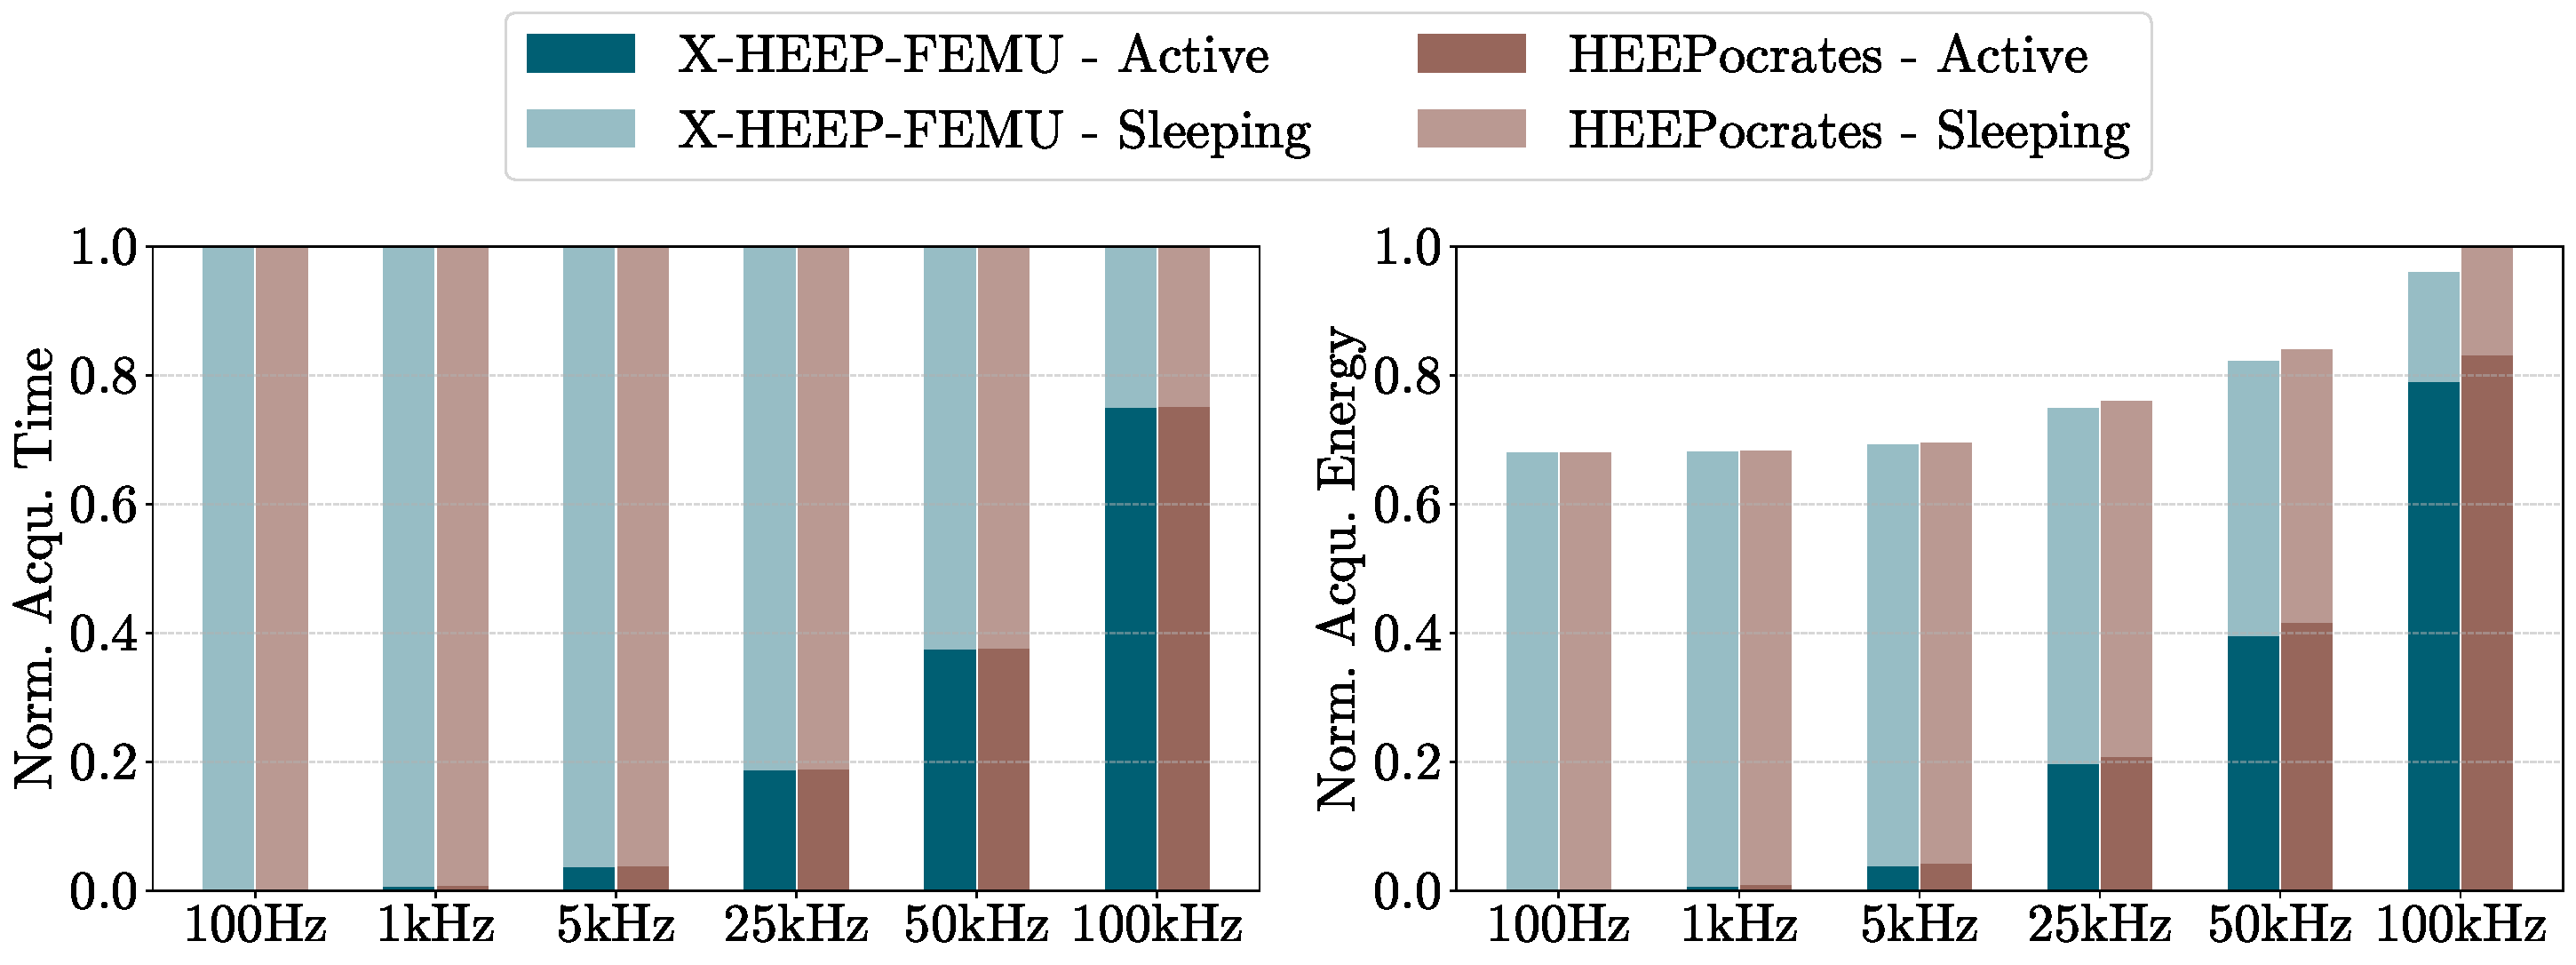
\includegraphics[width=1\textwidth]{./figures_femu/acquisition.pdf}
                \caption{Normalized acquisition time and energy on the \mbox{X-HEEP-FEMU} platform and the \mbox{HEEPocrates} chip for a \SI{5}{\second} acquisition window, with sampling frequency varying from \SI{100}{\hertz} to \SI{100}{\kilo\hertz}.}
                \label{fig:acquisition}
            \end{figure}

        \subsection{Computation of Typical TinyAI Workloads}
            
            Table~\ref{tbl:processing} and Figure~\ref{fig:processing} show the normalized processing time and energy results for each kernel on both the \mbox{X-HEEP-FEMU} platform and the fabricated \mbox{HEEPocrates} chip. For each configuration, the relative contributions of different subsystems to total time and energy are reported, enabling detailed analysis.
            
            The introduction of the CGRA yields significant performance gains across all benchmarks. For the MM and FFT kernels, CGRA-based execution reduces total processing time by approximately \SI{5}{\times} and \SI{7}{\times}, respectively. However, the most substantial gain is observed in the CONV benchmark, where performance improves by nearly \SI{9}{\times}. This enhancement can be attributed to the high computational intensity and spatial regularity of convolution operations, which are particularly well-suited to reconfigurable dataflow accelerators. These results demonstrate the potential of spatial accelerators to boost throughput and responsiveness in edge devices.

            \begin{table}[tp]
                \caption{Normalized processing time (in cycles) and power consumption (in \si{\milli\watt}) across platforms and processing elements for representative workloads.}
                \label{tbl:processing}
                \centering
                \resizebox{0.85\textwidth}{!}{
                \begin{tabular}{|l|c|c|c|c|}
                \toprule
                \bf{Workload} & \bf{Platform} & \bf{Proc. Element} & \bf{Proc. Time [cc]} & \bf{Power [\si{\milli\watt}]} \\
                \midrule
                MM   & X-HEEP-FEMU & CPU  & 83427 & 61.2 \\
                     & HEEPocrates & CPU  & 83427 & 64.3 \\
                     & X-HEEP-FEMU & CGRA & 11375 & 90.4 \\
                     & HEEPocrates & CGRA & 11375 & 108 \\
                \midrule
                FFT  & X-HEEP-FEMU & CPU  & 230841 & 54.0 \\
                     & HEEPocrates & CPU  & 230841 & 56.7 \\
                     & X-HEEP-FEMU & CGRA & 45331 & 87.0 \\
                     & HEEPocrates & CGRA & 45331 & 104 \\
                \midrule
                CONV & X-HEEP-FEMU & CPU  & 564968 & 54.0 \\
                     & HEEPocrates & CPU  & 564968 & 56.7 \\
                     & X-HEEP-FEMU & CGRA & 61276 & 116 \\
                     & HEEPocrates & CGRA & 61276 & 140 \\
                \bottomrule
                \end{tabular}
                }
            \end{table}
            
            Beyond performance, CGRA acceleration also consistently improves energy efficiency. The reduction in execution time directly translates into lower energy consumption, as dynamic power is amortized over a shorter period. Compared to CPU-only configurations, energy savings range from \SI{3}{\times} to \SI{6}{\times} depending on the kernel, highlighting the benefits of hardware offloading.
            
            Importantly, the energy trends observed on the FPGA-based \mbox{X-HEEP-FEMU} platform closely match those measured on the \mbox{HEEPocrates} chip. For CPU-only configurations, the average deviation between the two platforms is approximately \SI{5}{\percent}, demonstrating the accuracy of the energy estimation strategy based on pre-characterized power models. In CGRA-accelerated scenarios, the deviation increases to about \SI{20}{\percent}. This is primarily due to the use of power values extracted from post-layout reports for the CGRA, which are less precise than silicon measurements. Nonetheless, the deviations remain within acceptable bounds for architectural exploration.
            
            Overall, these results confirm the ability of the \mbox{X-HEEP-FEMU} framework to capture realistic performance and energy trends in complex TinyAI processing workloads. This confirms its suitability for hardware/software co-design and accelerator evaluation.
    
        \subsection{Sample Collection and Storage}
        
            To further highlight the benefits of the virtualization mechanisms provided by the \mbox{X-HEEP-FEMU} framework, a third use case focused on large-scale sample collection and storage is considered. This experiment is drawn from a real-world application introduced in~\cite{moisture}, which addresses the problem of classifying wood moisture levels using acoustic signal analysis. In such machine learning-driven sensor applications, efficient acquisition and storage of large datasets are critical to enable robust training and inference across diverse environmental conditions.
            
            In this use case, each acquisition window comprises 35,000 ultrasound samples captured at \SI{16}{\bit} resolution, totaling over \SI{70}{\kibi\byte} per window. Traditionally, these data are stored on board using physical non-volatile memory, such as SPI flash. However, such storage introduces significant latency due to limited bandwidth and access overheads.

            \begin{figure} [t]
                \centering
                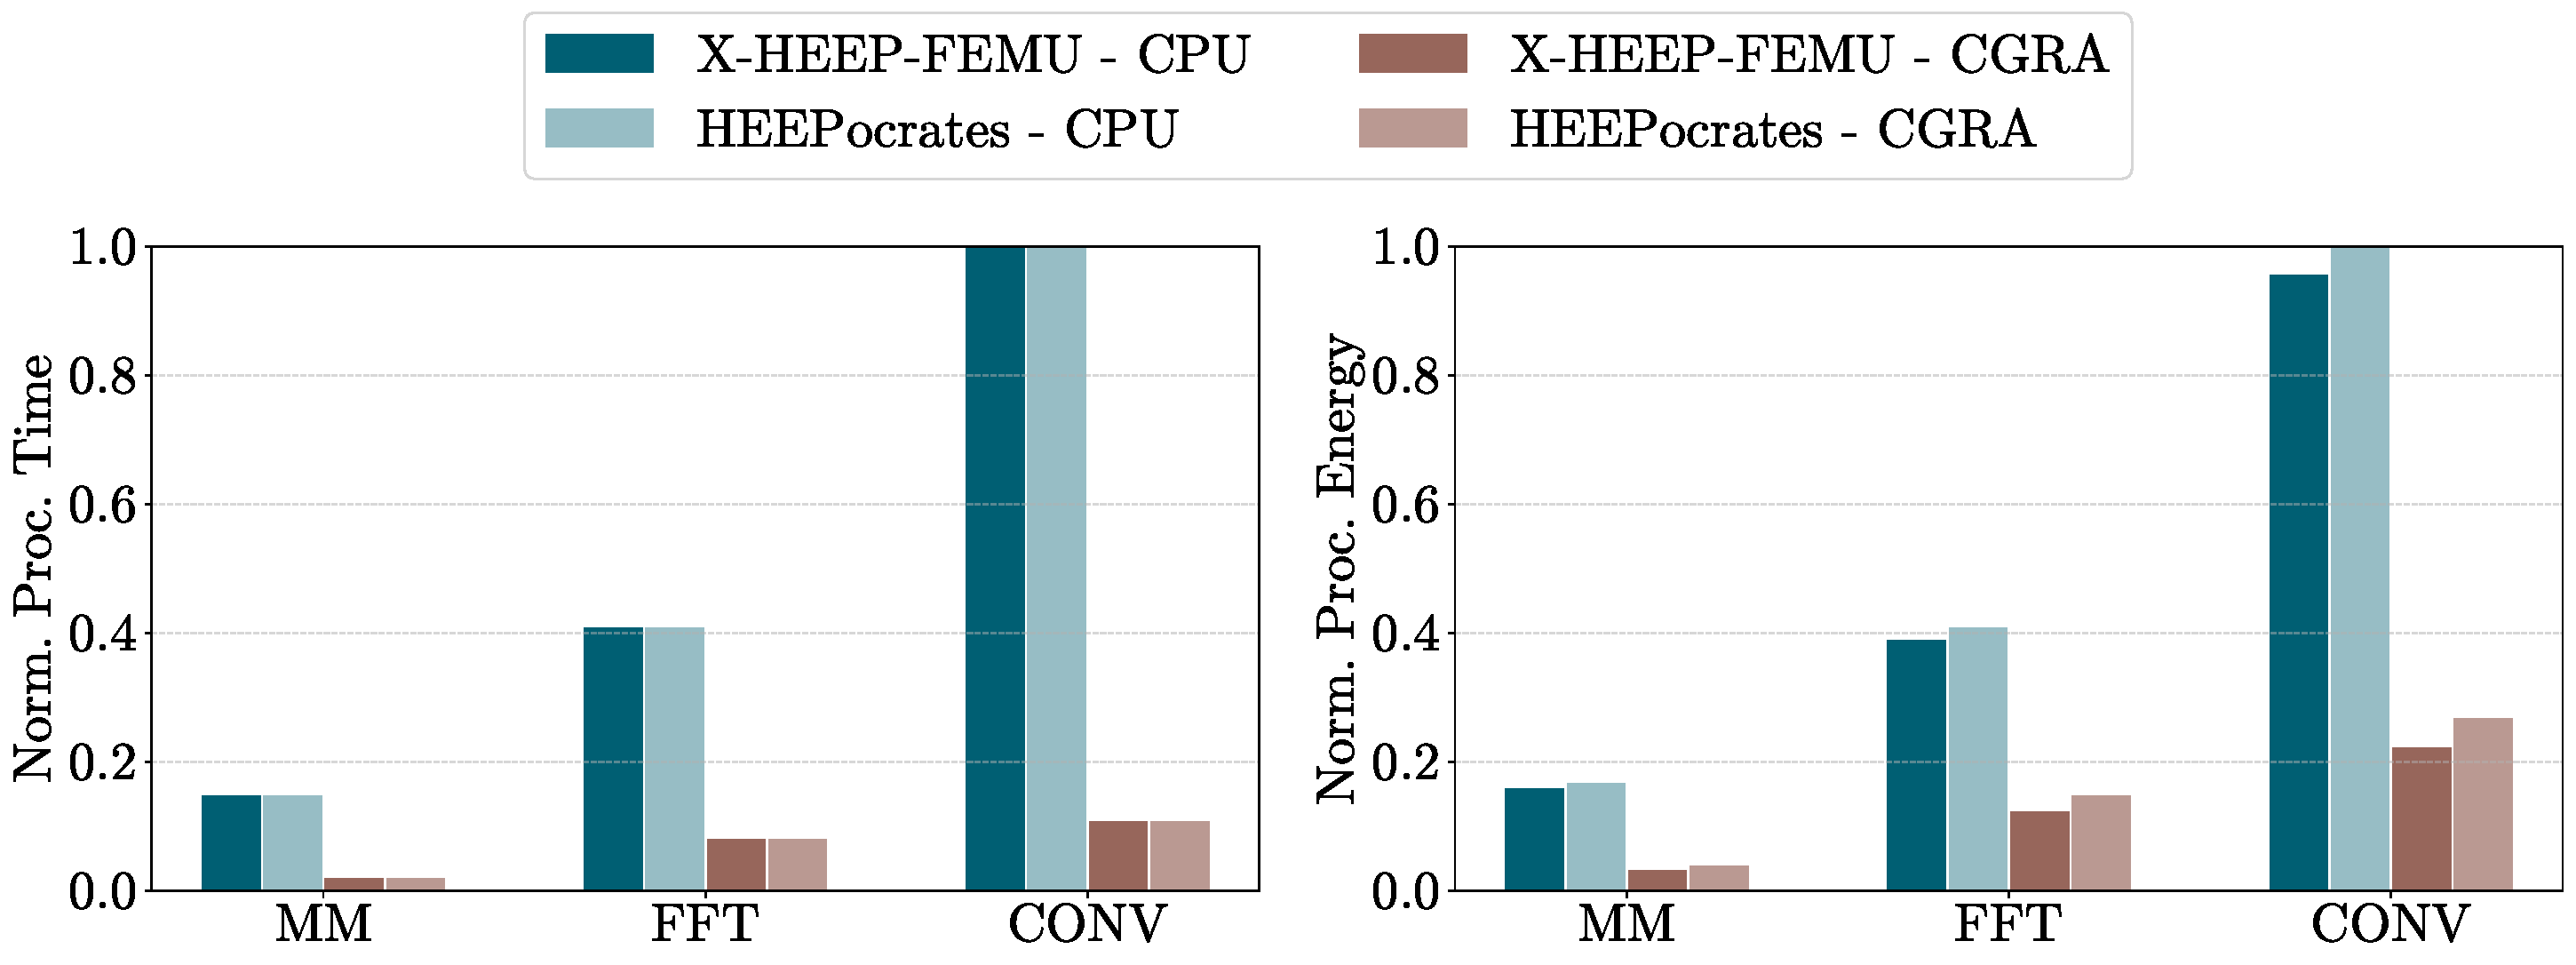
\includegraphics[width=1\textwidth]{./figures_femu/processing.pdf}
                \caption{Normalized processing time and energy on the \mbox{X-HEEP-FEMU} platform and the \mbox{HEEPocrates} chip for three representative kernels executed on both the CPU and the CGRA accelerator.}
                \label{fig:processing}
            \end{figure}
            
            The experiment leverages the flash virtualization capability of \mbox{X-HEEP-FEMU} to eliminate these bottlenecks. Instead of streaming data through a physical flash interface, the platform uses a virtualized SPI-to-AXI bridge to redirect read and write transactions to the PS, where they are mapped to high-speed DRAM managed by the ARM processor, as described in Section~\ref{sec:an_implementation}. This allows samples to be transferred directly between the host system and off-chip storage via the standard memory hierarchy, bypassing physical flash delays. Table~\ref{tbl:flash_virtualization} summarizes the obtained results.
            
            The measured acquisition time highlights the significant advantage offered by flash virtualization. With a physical flash device, each data window requires approximately \SI{2.5}{\second} to be transferred, resulting in a total duration of over \SI{10}{\minute} for a full experiment consisting of 240 windows. In contrast, when virtualization is enabled, the same data can be transferred in less than \SI{10}{\milli\second} per window, reducing the total acquisition time to just \SI{2.4}{\second}. This translates to a \SI{250}{\times} speedup, substantially improving system responsiveness and enabling large-scale data collection within seconds.
            
            This experiment underscores the key role of flash virtualization in enabling scalable data-driven workloads on ultra-low-power platforms. The ability to transfer large datasets quickly and reliably is essential for supporting machine learning workflows, where repeated acquisition, labeling, and inference are required.
        
    \section{Summary and Conclusions}
    \label{sec:conclusions}
    
        This chapter has introduced \mbox{FEMU}, an open-source and configurable emulation framework designed to enable the rapid prototyping and evaluation of TinyAI heterogeneous systems. Built upon the capabilities of SoC-based FPGAs, \mbox{FEMU} bridges the gap between early-stage development and realistic evaluation by combining an RH region, where the heterogeneous system is implemented, with a CS region that runs a full operating system. This architecture enables flexible, real-time interaction between software and hardware components while maintaining the accuracy and realism required to guide system-level design decisions.
        
        The motivation behind the framework was established through an analysis of limitations found in existing RTL-based and software-based solutions, as well as recent FPGA-based prototyping platforms. Although several prior works address aspects such as performance monitoring, modularity, or low-power execution, none provide a unified solution that combines heterogeneous systems-based design, OS-level control, dynamic IP virtualization, and accurate performance and energy estimation. \mbox{FEMU} addresses this gap by integrating all these capabilities within a cohesive and extensible platform tailored to the constraints of the TinyAI domain.

        \begin{table}[tp]
            \caption{Acquisition time comparison with and without flash virtualization.}
            \label{tbl:flash_virtualization}
            \centering
            \resizebox{1\textwidth}{!}{
            \begin{tabular}{|l|c|c|c|}
            \toprule
            \bf{Configuration} & \bf{Per-Window Transfer Time} & \bf{Total Duration (240 Windows)} & \bf{Speedup} \\
            \midrule
            Physical Flash Storage & \SI{2.5}{\second} & \SI{10}{\minute} & \textemdash \\
            Virtualized Flash & $<$\SI{10}{\milli\second} & \SI{2.4}{\second} & \SI{250}{\times} \\
            \bottomrule
            \end{tabular}
            }
        \end{table}
        
        The architectural details of the framework, including its key hardware and software components and associated features, were described. The implementation of a debugger, ADC, flash, and accelerator virtualization enables early-stage development without requiring physical integration. In addition, performance and energy evaluations are supported by a lightweight monitoring infrastructure and energy models derived from real silicon measurements.
        
        A structured prototyping and evaluation flow was presented to guide the identification, modeling, and integration of hardware accelerators. This iterative methodology facilitates incremental improvements in performance and energy efficiency while preserving functional correctness and reducing development time.
        
        To demonstrate the methodology in practice, the \mbox{X-HEEP-FEMU} platform was instantiated using real hardware and software components. The platform was deployed on the Xilinx Zynq-7020 SoC, integrating the \mbox{X-HEEP}~\cite{x-heep} host in the PL, a Linux-based Python environment on the ARM Cortex-A9 PS, and energy models derived from a TSMC \SI{65}{\nano\meter} CMOS implementation of \mbox{X-HEEP}, referred to as \mbox{HEEPocrates}~\cite{heepocrates}. This instantiation validates the applicability of the \mbox{FEMU} framework in real-world scenarios.
        
        The \mbox{X-HEEP-FEMU} platform was evaluated across a series of representative use cases. The experimental campaign demonstrated strong alignment with silicon-based measurements, confirming both timing fidelity and accurate energy estimation. In particular, the following quantitative outcomes were obtained:

        \vspace{-1em}
        \begin{itemize}
            \item \textbf{Signal acquisition characterization:} Data acquisition often dominates TinyAI system activity during long idle phases, making accurate modeling of peripheral behavior and energy use essential. This experiment verified that the ADC virtualization infrastructure replicates real-time sampling and power patterns across a wide frequency range. For a \SI{5}{\second} window, emulation matched silicon timing exactly, with energy errors below \SI{5}{\percent}, and reproduced the shift from sleep-dominated operation at \SI{100}{\hertz} (CPU active less than \SI{1}{\percent}) to active-dominated at \SI{100}{\kilo\hertz} (CPU active more than \SI{70}{\percent}), confirming its ability to model duty-cycle-dependent energy behavior.
        
            \item \textbf{Computation of typical TinyAI workloads:} Core kernels such as matrix multiplication, convolution, and FFT were evaluated in CPU-only and CGRA-accelerated modes to quantify performance and energy gains. CGRA execution improved performance by approximately \SI{5}{\times} for MM, \SI{7}{\times} for FFT, and nearly \SI{9}{\times} for CONV, with energy reductions of \SI{3}{\times} to \SI{6}{\times}. Energy trends matched silicon within \SI{5}{\percent} for CPU-only mode and about \SI{20}{\percent} for CGRA mode, supporting its use for accelerator trade-off studies.
        
            \item \textbf{Sample collection and storage:} Many TinyAI applications require efficient dataset storage, yet physical flash introduces bandwidth and latency bottlenecks. Flash virtualization removed these constraints, reducing per-window transfer from \SI{2.5}{\second} to less than \SI{10}{\milli\second}, achieving a \SI{250}{\times} speedup and cutting 240-window acquisition from more than \SI{10}{\minute} to \SI{2.4}{\second}, enabling rapid, large-scale dataset collection in development and testing.
        \end{itemize}
        \vspace{-1em}
 
        In conclusion, \mbox{FEMU} provides a flexible, extensible, and realistic environment for the development and evaluation of heterogeneous systems in the TinyAI domain. Its support for early-stage experimentation through virtualization, seamless accelerator integration, and accurate performance and energy assessment enables rapid iteration and informed design decisions. As a result, \mbox{FEMU} significantly reduces development effort and risk, representing a critical advancement in the prototyping of next-generation ultra-low-power intelligent systems.
